%
% このファイルは、筑波大学大学院システム情報工学研究科の
% 学位論文本体のサンプルです。
% このファイルを書き換えて、この例と同じような書式の論文本体を
% LaTeXを使って作成することができます。
% 
% PC環境や、LaTeX環境の設定によっては漢字コードや改行コードを
% 変更する必要があります。
%%
\documentclass[a4paper,11pt]{jreport}

%%【PostScript, JPEG, PNG等の画像の貼り込み】
%% 利用するパッケージを選んでコメントアウトしてください。
%\usepackage{graphicx} % for \includegraphics[width=3cm]{sample.eps}
\usepackage{epsfig} % for \psfig{file=sample.eps,width=3cm}
%\usepackage{epsf} % for \epsfile{file=sample.eps,scale=0.6}
%\usepackage{epsbox} % for \epsfile{file=sample.eps,scale=0.6}

%% dvipdfm を使う場合(dvi->pdfを直接生成する場合)
%\usepackage[dvipdfm]{color,graphicx}
%% dvipdfm を使ってPDFの「しおり」を付ける場合
%\usepackage[dvipdfm,bookmarks=true,bookmarksnumbered=true,bookmarkstype=toc]{hyperref}
%% 参考:dvipdfm 日本語版
%% http://hamilcar.phys.kyushu-u.ac.jp/~hirata/dvipdfm/

%自分で入れた物
\usepackage{color}
\usepackage{url}
\usepackage{algorithm}
\usepackage{algorithmic}
\usepackage{}

%手法名
\newcommand{\SysName}{\$V}

% 修正とTODO
\newcommand{\fixme}[1]{\textcolor[rgb]{1,0,0}{#1}}
\newcommand{\TODO}[1]{\textcolor[rgb]{0,0,1}{#1}}

% 参照
\newcommand{\refImg}[1]{図\ref{img:#1}}
\newcommand{\refSec}[1]{\ref{sec:#1}節}
%\newcommand{\refSec}[1]{第\ref{sec:#1}節}
\newcommand{\secLabel}[1]{\label{sec:#1}}

% 画像
\newcommand{\img}[5]{
\begin{figure}[#1]
	\begin{center}
		\includegraphics[width = #2\hsize]{./img/#3}
	\end{center}
	\caption{#4}
	\label{img:#5}
\end{figure}
}

\newcommand{\unit}[1]{\,#1} % 120,\unit{mm}→120mm」をイイ!感じにスペーシングしてくれる
\newcommand{\kake}{~$\times$~} % →×

\usepackage{times} % use Times Font instead of Computer Modern

\setcounter{tocdepth}{3}
\setcounter{page}{-1}

\setlength{\oddsidemargin}{0.1in}
\setlength{\evensidemargin}{0.1in} 
\setlength{\topmargin}{0in}
\setlength{\textwidth}{6in} 
%\setlength{\textheight}{10.1in}
\setlength{\parskip}{0em}
\setlength{\topsep}{0em}

%\newcommand{\zu}[1]{{\gt \bf 図\ref{#1}}}
 
%% タイトル生成用パッケージ(重要)
\usepackage{sie-jp-euc}
%% タイトル
%% 【注意】タイトルの最後に\\ を入れるとエラーになります
\title{ユーザ定義手書きジェスチャの高速かつ軽量な認識アルゴリズム}
%% 著者
\author{山路 大樹}
%% 学位 (2012/11 追加)
\degree{修士(工学)}
%% 指導教員
\advisor{志築 文太郎}

%% 専攻名 と 年月
%% 年月は必要に応じて書き替えてください。
%\majorfield{コンピュータサイエンス} \programfield{} \yearandmonth{2017年 3月}
\majorfield{コンピュータサイエンス} \yearandmonth{2017年 3月}



\begin{document}
\maketitle
\thispagestyle{empty}
\newpage

\thispagestyle{empty}
\vspace*{20pt plus 1fil}
\parindent=1zw
\noindent
%%
%% 論文の概要(Abstract)
%%
\begin{center}
{\bf 概要}
\vspace{5mm}
\end{center}

ペンや指を用いた手書きジェスチャを入力として用いるアプリケーション
手書きジェスチャを認識するための既存アルゴリズムは専門的な知識が必要であったり,認識させるための必要な学習データの数が膨大であったりする.\$1は,アルゴリズムが簡潔である,少ない学習データにおいて高い認識率を示す,認識速度が速い,ロバスト性が高いと行った特徴を持つ手書きジェスチャ認識のためのアルゴリズムであり,様々な開発環境において,アプリケーション開発初学者を含む多くの開発者によって利用されてきた.しかしながら,ユーザ調査により,アプリケーションユーザは,手書きジェスチャの形状や書き順が同じでも,大きさ,向き,位置の違いを利用したジェスチャを入力したいという要望があることがわかった.\$1を始め\$1を改良した多くのアルゴリズムは,認識率や認識速度の低下を危惧し,これらの手書きジェスチャを識別できるように実装されていない.
そこで本論文にて,認識率や認識速度の低下を最小限に抑えつつ,手書きジェスチャの形状や書き順が同じでも,大きさ,向き,位置に関して識別可能なをアルゴリズム\$V示す.\$Vは保管されている学習データの類似度をもとに,類似度計算するジェスチャを選び,認識に用いる特徴量に重み付けすることによって,認識率及び認識速度の低下を抑えた.アプリケーション開発者は,本論文において示されるアルゴリズムを自身のシステムに組み込むことにより,大きさ,向き,位置の違いを利用したジェスチャを入力として用いるようなアプリケーションを開発することができる.
また,\$Vの性能評価のために既存アルゴリズムとの比較実験を行い,その結果から\$Vの有用性を示した.

%%%%%
\par
\vspace{0pt plus 1fil}
\newpage

\pagenumbering{roman} % I, II, III, IV 
\tableofcontents
\listoffigures
%\listoftables

\pagebreak \setcounter{page}{1}
\pagenumbering{arabic} % 1,2,3

%序論
\chapter{序論}
本研究にて,ユーザが定義した手書きジェスチャを高速に認識し,かつ容易に実装可能な軽量なアルゴリズムを示す.
本章にて,まず初めに研究背景として既存の手書きジェスチャ認識手法とその課題を述べる.次にその課題を解決すべく本研究の目的を述べ,最後に本論文の構成を述べる.

\section{背景}
スマートフォンやタブレット端末のタッチパネルへの入力手法として,ペンや指を用いた手書きジェスチャが多く採用されている.特にそれらを入力として用いるようなアプリケーションをプロトタイピングする環境において,手書きジェスチャをアプリケーションに組み込む際に求められることとして,~\cite{Rettig:1994:PTF:175276.175288}において述べられているように,手書きジェスチャ認識を実現するためのパターン認識に関する専門的な知識~\cite{Hong00constructingfinite, Anderson2004HiddenMM,Sezgin:2005:HES:1040830.1040899, Cao:2005:EOA:1089508.1089540, Pittman:1991:RHT:108844.108914, Cho:2006:NGR:1711617.1711649,Rubine:1991:SGE:127719.122753, Anthony:2010:LMR:1839214.1839258}がなくとも,素早く実装できること(すなわち複雑な数式やアルゴリズムを用いていないということ),素早く手書きジェスチャ入力のテストができること(すなわちあまり学習データを必要としないこと)などが挙げられる.同時に,ジェスチャ認識であるため,認識率が高いこと,認識速度が速いことも求められる.また,手書きジェスチャは,入力されるジェスチャの形状が毎回微妙に異なる可能性が高いため,たとえ形状が微妙に異なったとしても意図したジェスチャとして正しく認識されるようなロバスト性の高い認識アルゴリズムであることも求められる.また,学習データをあまり必要としないということは,アプリケーションユーザが独自に手書きジェスチャを定義することが可能なシステムを実現することにもつながり,これも手書きジェスチャを入力として用いるアプリケーションを開発する多くの開発者によって求められていることの1つである.

\$1~\cite{Wobbrock:2007:GWL:1294211.1294238}は,まさにこれらの要件を満たす手書きジェスチャ認識アルゴリズムであり,「アルゴリズムが簡潔である,少ない学習データにおいて高い認識率を示す,認識速度が速い,ロバスト性が高い」といった特徴を持ち,単一ストロークからなる手書きジェスチャを認識可能なアルゴリズムである.\$1は,現に,ActionScript, Python, C\#, C++, Objective-C, Java, Java ME, and JavaScriptといった言語において実装されている.
そのため,多くの開発者にとって,手書きジェスチャ認識を自身のシステムに組み込むことが容易となった.特に手書きジェスチャ認識のためのライブラリが存在しないようなプロトタイピング開発環境において,その存在価値は非常に高い.また,\$1を改良した多くのアルゴリズムは\$-Family Recognizer~\cite{Anthony:2010:LMR:1839214.1839258,Reaver:2011:MQU:2021164.2021183,Li:2010:PFA:1753326.1753654,Anthony:2012:NFA:2305276.2305296,Herold:2012:CRF:2331067.2331074,Vatavu:2012:GPC:2388676.2388732,Taranta:2015:PPB:2788890.2788925,Pittman:2016:FFA:2856767.2856808,Vatavu:2012:OAF:2166966.2167022}として知られ,\$1の持つ「アルゴリズムが簡潔である」という特徴を維持しつつ,認識率や認識速度の向上,識別可能なジェスチャの種類の増加といった観点から改良が試みられた.ペンや指を入力として用いるようなインタフェースが普及し,それらを用いたアプリケーションの開発者が増加している今日において,これらアルゴリズムは,手書きジェスチャ認識を自身のシステムに容易に組み込むための手段として必要とされており,アルゴリズムの開発・改良の機運が高まっている.
これまで開発されてきた\$-Family Recognizerは,ジェスチャを構成するストロークの,大きさ,向き,位置に関して,そのいずれかあるいはすべてについて不変になるようなアルゴリズムを採用することにより,不変にしたものについてロバストなジェスチャ認識を実現した.大きさ,向き,位置に関して不変にするということは,
%これらアルゴリズムにおいては,
手書きジェスチャの書き順が同じでありかつ手書きジェスチャの形状さえ類似していれば,ジェスチャの大きさ,向きあるいはジェスチャが入力された位置などが多少異なっても,同じ形状と書き順の手書きジェスチャとして認識されるということである.その結果,認識率の向上が実現された.
それらを不変にしない,つまり特徴量として認識のために用いるということは,その特徴量について識別できるため,識別可能な手書きジェスチャが増加することにつながるが,不変にしない特徴量についてはロバストではなくなるため,認識率の低下を招く恐れがある.
例えば,Rubine Classfier~\cite{Rubine:1991:SGE:122718.122753}は13もの手書きジェスチャの特徴量を用いることにより手書きジェスチャを認識し,手書きジェスチャを構成するストロークの形状と書き順は同じであるが,大きさ,向き,位置に関して異なるジェスチャ~(図\ref{fig:examples_V})を識別することが可能である.しかしながら,認識に用いる特徴量が多いため,結果的に認識率の低下を招いている.

\begin{figure} [htbp]
\centering
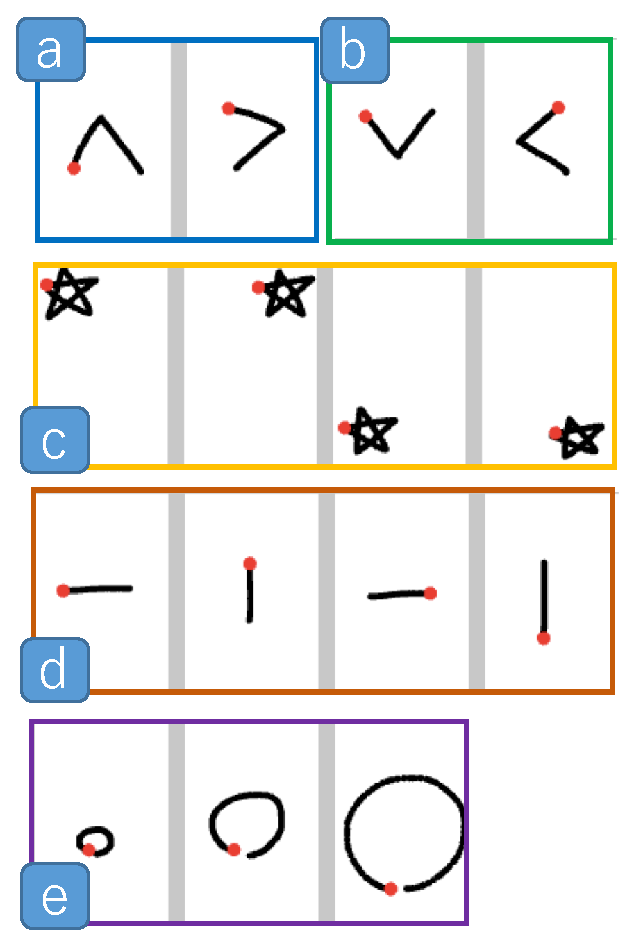
\includegraphics [width=0.5\columnwidth]{img/examples_V.eps}
\caption{ジェスチャの形状と書き順は同じであるが,向き (a) (b) (d),位置 (c),大きさ (e)が異なる,単一ストロークからなる手書きジェスチャの例.}
\label{fig:examples_V}
\end{figure}


認識速度の観点でいえば,DTW~\cite{Tappert:1982:CSR:1664966.1664979, Salvador:2007:TAD:1367985.1367993}は,手書きジェスチャ認識を実現するために広く採用されているアルゴリズムであり,単純にストロークを構成する点の距離を比較するのみであるため,こちらも,手書きジェスチャを構成するストロークの形状と書き順は同じであるが,大きさ,向き,位置に関して異なるジェスチャを識別することは可能である.しかしながら,単純なアルゴリズムによって認識率を向上させるために,非常に計算量が大きいといった問題点がある.

しかしながら,ユーザ調査により,これまでに述べたきたような,ジェスチャの形状と書き順は同じであるが,大きさや向きや位置が異なる単一ストロークからなる手書きジェスチャ~(図\ref{fig:examples_V})をアプリケーションユーザが入力として用いることを要望していることが導かれた.
これらは既に述べたように既存の\$-Family Recognizerにおいて識別できないため,ユーザが定義するこれらのような手書きジェスチャを入力として用いるようなアプリケーションを開発したい開発者は既存の\$-Family Recognizerを認識アルゴリズムとして用いることができない.また,これらを識別可能なRubine classfierやDTWなどを採用した場合は,認識率や認識速度において十分なパフォーマンスを得られない可能性がある.


\section{目的}
本研究の目的は,\$1を拡張し,単一ストロークからなる手書きジェスチャに対し,ジェスチャの大きさ,向き,位置に関して識別可能としながらも,\$1と比較し認識率の低下と認識速度の低下を最小限に抑えることを実現した\$-Family Recognizer開発することである.
我々はこの,ジェスチャの大きさ,向き,位置に関して``V''ariant~(不変)な手書きジェスチャを認識する\$-Family Recognizerを\$Vと名付けた.
\$Vは\$1に簡単な数式からなるアルゴリズムを追加することによって,どのような開発環境においても実装可能なアルゴリズムを開発することも目標としている.
また,\$1と同様,少ない学習データにおいて高い認識率を示すことも目標としており,これは,アプリケーションユーザが手書きジェスチャを独自に定義することが可能であることを示している.
また,大きさ,向き,位置に関して識別可能な既存アルゴリズムと比較することによって,\$Vの有用性を示すことも本研究における目的とする.


%\$Vは,大きさ,向き,位置を特徴量として用いることによって,それらに依存するストロークを識別可能とした.
%その際,学習データを元に,ストロークを形状と書き順ごとに分類し,認識に用いる特徴量に重み付けをすることによって考慮すべき特徴量を適切に配分し,\$1と比べても遜色のない認識率と認識速度を実現した.
%\$1を改良した多くのアルゴリズムを用いず,\$1を拡張した理由は,\$1にて計算された,大きさ,向き,位置の特徴量を再利用することによって,\$1アルゴリズムと比べて,アルゴリズムの追加量を抑えること,認識速度の低下を抑えることにつながるからである.

\section{貢献}
本研究における手書きジェスチャ認識アルゴリズム\$Vの貢献を以下に示す.
\begin{itemize}
\item 手書きジェスチャを構成するストロークの形状と書き順は同じであるが,大きさ,向き,位置に関して異なる手書きジェスチャを識別することが可能なアルゴリズムを開発した.
\item 少ない学習データにおいて認識率を向上させるためのアルゴリズムを開発した.
\item 認識速度を向上させるためのアルゴリズムを開発した.
\item 実装が容易な軽量なアルゴリズムを開発した.
\end{itemize}

\section{本論文の構成}
第1章では,研究背景と目的を述べた.第2章では,関連研究を述べる.第3章では,本研究の動機にもなった,アプリケーションユーザが入力として用いたい手書きジェスチャの調査を述べる.第 4 章では,\$Vの拡張元である\$1アルゴリズムを述べ,第5章において,\$Vのアルゴリズムの詳細を述べる.第6章では,\$Vのアルゴリズムとしての性能評価実験を述べる.第7章では,\$Vを用いたアプリケーション例を述べる.第8章では,\$Vアルゴリズムの改善点と今後の展望を議論する.第9章では,本研究の結論を述べる.
なお,付録 A に\$Vアルゴリズムの擬似コードを示す.
%付録 B に第 3章のユーザ調査に用いた調査同意書を,付録 B に調査について説明する際に用いた説明書を,付録 Dに第6章の評価実験に用いた実験同意書を示す.


%関連研究
\chapter{関連研究}
本章にて,本研究に関連する研究を述べる.本研究では,ユーザが定義する手書きジェスチャを高速に認識し,かつ容易に実装可能な軽量なアルゴリズムを開発している.また,本研究において開発したアルゴリズム\$Vはストロークの大きさ,向き,位置に関して識別可能な\$-Family Recognizerである.以上を踏まえ,本研究の関連研究を,一般的な手書きジェスチャ認識アルゴリズムの研究,ユーザ定義に特化した手書きジェスチャ認識アルゴリズムの研究,Progamming by Exampleに関する研究,\$-Family Recognizerに関する研究,手書きジェスチャ認識を可能にするツールキットに関する研究,手書きジェスチャの評価に関する研究に分類する.
本章にて,それらの研究について述べた後,最後に本研究における手書きジェスチャ認識アルゴリズムである\$Vの位置づけについて述べる.

\section{手書きジェスチャ認識アルゴリズム}
文字,ストロークの形状,手書きジェスチャなどの認識は,長く広く研究されている分野であり,多くのアルゴリズムにより実現されてきた.
finite state machines~\cite{Hong00constructingfinite}~(有限オートマトン)は,有限個の状態と遷移と動作の組み合わせからなる論理モデルであり,ある「状態」において,何らかのイベントや条件によって別の状態へ「遷移」することを繰り返すことによって最終的な認識結果を導く.高い認識精度を示すためには,より詳細なモデルの定義が必要となる.
Hidden Markov Models~(HMMs)~\cite{Anderson2004HiddenMM,Sezgin:2005:HES:1040830.1040899, Cao:2005:EOA:1089508.1089540}~(隠れマルコフモデル)は,観測された出力の系列から,内部の状態系列を統計的に推測するためのアルゴリズムである.
neural networks~\cite{Pittman:1991:RHT:108844.108914}は脳機能の特性を計算機上に応用したアルゴリズムであり,大量の学習によってモデルを最適化し,多次元量のデータで線形分離不可能な問題に対して比較的小さい計算量で良好な解を得ることができる.
feature-based statistical classifiers~\cite{Cho:2006:NGR:1711617.1711649,Rubine:1991:SGE:127719.122753}は,大量の学習データによる特徴量をもとに学習データをクラスタリングし,より低次元な認識モデルを生成するためのアルゴリズムである.
ad hoc heuristic recognizers~\cite{Anthony:2010:LMR:1839214.1839258, Wilson:2003:XUI:642611.642706}は,「限定的な」認識アルゴリズムであるため,事前に定義されたジェスチャのみ認識することができる.すなわち,アプリケーション実行時において,新たな学習データを追加した場合に,新たなヒューリスティック関数を定義しなければならないため,アプリケーションユーザが独自にジェスチャを定義することができない.
template matching~\cite{Kara:2005:ITS:1652319.1652712, Kristensson:2004:SLV:1029632.1029640}は.主に画像処理に利用され,学習データと入力データの画像をそれぞれ走査し,画像上の各位置における類似度を算出するアルゴリズムであり,手書き文字にも応用されている.

これらアルゴリズムはオンライン文字認識及びオフライン文字認識双方においてしばしば用いられるアリゴリズムである.オンライン文字認識とは,ディスプレイなどにペンや指などによって入力された文字を認識する技術の総称であり,オフライン文字認識とは,紙に書かれた文書イメージを光学スキャンし,そのイメージを自動的にコンピュータで処理可能なテキストデータに変換する技術の総称である.しかしながら,これらアルゴリズムは,高い認識精度を示す認識モデルを生成するために膨大な数の学習データが必要であり,素早く手書きジェスチャ入力のテストしたい場合において不向きであるだけでなく,アプリケーションユーザが独自にジェスチャを定義する上で実用的であるとは言えない.また,これらアルゴリズムを実装することは,それぞれの分野に精通していない開発者にとって困難である.

\section{ユーザ定義に特化した手書きジェスチャ認識アルゴリズム}
ユーザ定義の手書きジェスチャを認識できるアルゴリズムのうち,少ない学習データによって高い認識率を示すアルゴリズムを示す.
Rubine classifier~\cite{Rubine:1991:SGE:122718.122753}及びDynamic programming~(DTW)~\cite{Tappert:1982:CSR:1664966.1664979}などは,少ない学習データにおいてジェスチャ認識可能なアルゴリズムであるが,Rubine classifierはアルゴリズムに用いられる数式が複雑である上,学習データが2つの場合は認識率が高いとは言えない.また,DTWはアルゴリズムが簡潔であるが,計算量が非常に大きいという問題点がある.計算量を改善したFast DTW~\cite{Salvador:2007:TAD:1367985.1367993}が開発されたが,アルゴリズムは複雑になっており,プロトタイピング環境開発向けとは言い難い.
また,Rubine classifierは多くある特徴量を適切に選ばないと,認識率が低下するという欠点があり,それぞれの特徴量が認識結果に及ぼす影響について深い知識がない場合,特徴量の選定が難しい.このように認識に用いる特徴量を単に増やすことは,それについて識別できることにつながるが,ロバスト性の低下を招くという欠点もある.

\section{Programming by Example}
Programming by Exampleとは,学習データをもとに,認識モデルを自動生成する手法である.
システムに明示的に学習データを例として与え,ユーザの意図や好みを推論することにより,ユーザの意図に沿った処理を行ったり,処理自体を削減したりすることが可能となる~\cite{110003743975}.この手法は手書きジェスチャ認識においても活用されている.
Tarantaら~\cite{Taranta:2016:RPA:2984511.2984525}は,Gesture Path Stochastic Resampling~(GPSR)という,学習データをもとに人間が書くような手書きジェスチャを生成するためのアルゴリズムを考案した.このように,あるデータをもとにそのデータにより近く,より自然な新たなデータを自動生成するアルゴリズムとして,Syntetic Data Generation~(SDG)~\cite{conf/iccv/NavaratnamFC07,Shotton:2011:RHP:2191740.2192047,Galbally_syntheticgeneration,Lundin:2002:SFD:646280.687684,Gatos:2005:SAK:1106779.1106876,Rodriguez-Serrano:2012:SQH:2240326.2240755,Fischer:2013:GLS:2501115.2501123}があり,これらのアルゴリズムは手書きジェスチャを始めとするパターン認識において用いられている.また,Perlin noise~\cite{Perlin:1985:IS:325165.325247}あるいは,SigmaLognormal~\cite{SigmaLognormal}も,手書きジェスチャを自動生成するためのアルゴリズムとして広く利用されている.GPSRはユーザから得られたそれぞれの手書きジェスチャの特徴をもとに,そのジェスチャの認識率が高くなるような自動生成方法を計算することによって,これらのアルゴリズムよりも高い認識率を示した.これらは,学習データを大量に自動生成することができるため,少ない学習データにおいて高い認識率を示す,ユーザ定義に特化した手書きジェスチャ認識アルゴリズムでもある.

\section{\$-Family Recognizer}
\$1~\cite{Wobbrock:2007:GWL:1294211.1294238}は,\$-Family Recognizerの先駆的なアルゴリズムであり,\$1を改良したアルゴリズムは,\$-Family Recognizerと呼ばれている.
\$1は,少ない学習データにより,高い認識率を示すアルゴリズムであるため,ユーザが独自にジェスチャを定義するジェスチャ認識システムを開発することが可能である.また,開発者は,自身のシステムに,簡単な数式のみを含む,およそ100行からなるアルゴリズムを追加するのみによって,単一ストロークからなるジェスチャ認識を行うことが可能であるため,手書きジェスチャ認識をプロトタイピングするような環境において実装可能である.\$1は入力データと学習データの対応する点のユークリッド距離が最小となるような最適な角度を探索することによってジェスチャ認識を行っている.
しかしながら,ストロークを,大きさ,向き,位置に不変にしているため,それらの特徴量に依存するようなジェスチャを認識することができない.したがって,そのようなジェスチャを認識するようなアプリケーションを開発したい開発者は\$1を自身のシステムに採用することができない.
\$1が認識することができないジェスチャを認識するために,これまで\$1を拡張した\$-Family Recognizerが開発されてきた.
\$N~\cite{Anthony:2010:LMR:1839214.1839258}は,複数のストロークからなるジェスチャを認識することを可能にし,識別可能なストロークを大幅に増やすことに成功した.\$Nは,ストロークを複数の単一ストロークに分割し,それぞれの単一ストロークを\$1の手法によって認識した.また,自動的に考えられる複数の単一ストロークの組み合わせを計算することによって,ストロークの向きや書く順番にロバストな認識も可能にした.
Quick\$~\cite{Reaver:2011:MQU:2021164.2021183}は,\$1の改良であり,最短距離法によるクラスタリングによって,対応する点のユークリッド距離が最小となる入力データと学習データの組み合わせを効率的に探索し,認識速度を高速化するアルゴリズムである.
Protractor~\cite{Li:2010:PFA:1753326.1753654}も\$1に対し,認識速度の面において改良した.最適な角度を探索する際に,Golden Section Search~(GSS)~\cite{Press:1992:NRC:148286}%(pp. 397-402)
を用いた\$1とは異なり,閉形式解を用いることによって,より高速に探索することを可能とした.
\$N-Protractor~\cite{Anthony:2012:NFA:2305276.2305296}は,\$Nに対し,Protractorの手法を用いることによって,より高速にかつ,より正確に複数のストロークからなるジェスチャを認識することを可能にした.
1 cent Recognizer~\cite{Herold:2012:CRF:2331067.2331074}は,\$1よりも高速であり,アルゴリズムも非常に単純であるため実装が容易であるが,認識・識別可能なジェスチャの種類や,認識率の観点から見るとあまり実用的であるとは言えない.
\$P~\cite{Vatavu:2012:GPC:2388676.2388732}は,ストロークを構成する点をPoint Cloudとして扱うことによって,\$N-Protractorよりも,メモリ消費量や認識速度の点において効率的なアルゴリズムである.
Penny Pincher~\cite{Taranta:2015:PPB:2788890.2788925}は,ストロークを構成する点間のベクトルを用いることによって,これまでの\$-Family Recognizerと比べて,より高速にかつ,正確に認識することを可能にした.

これらの\$-Family Recognizerは,2次元のストロークからなる手書きジェスチャを認識をすることが可能であり,\$1に対し,アルゴリズムを簡略化したり,認識速度を高速化したり,認識率を高くしたり,認識できるストロークの種類を増やしたりするなどして,繰り返し改善されてきた.

しかしながらこれらのアルゴリズムは,ストロークの特徴量である,大きさ,向き,位置に関して,そのいずれかあるいはすべてについて不変になるようなアルゴリズムを採用することにより,それらの特徴量についてロバストなジェスチャ認識を実現し,その結果認識率や,認識速度の向上を実現してきた.
それらを不変にしないことは,その特徴量について識別できるようになることにつながるが,不変にしない特徴量についてはロバストではなくなるため,認識率の低下や認識速度の低下を招く恐れがある.例えば,1 cent Recognizerはストロークを構成するすべての点の中心座標から,それぞれの点へのユークリッド距離のみを特徴量とし,入力データと学習データの特徴量の差が最小となるストロークを探索しているため,ストロークの形状と書き順は同じであるが,大きさ,向き,位置に関して異なるストロークを識別することは可能である.しかし,それぞれの特徴量についてロバストでないため,それぞれの特徴量について微妙に異なる場合,認識できないことが多々あり,結果的に認識率の低下を招いている.
%認識速度の観点でいえば,DTWは,単純にストロークを構成する点の距離を比較するのみであるため,こちらも,ストロークの形状は同じであるが,大きさ,向き,位置に関して異なるストロークを識別することは可能であるが,認識率を向上させるために,非常に計算量が大きい.

\section{手書きジェスチャ認識を可能にするツールキット}
%プロトタイピング環境向けに開発できるように,
手書きジェスチャ認識を簡単に開発することが可能なツールキットも開発された~\cite{Henry:1990:IGS:97924.97938,Landay:1993:EEU:259964.260123,Myers:1997:AEN:262050.260628}.SATIN~\cite{Hong:2000:STI:354401.354412}はジェスチャ認識の開発を容易にするだけでなく,ペンベースのユーザインタフェースを採用し,ジェスチャ認識のモデルを手書きによって定義することができるツールキットである.
%Henryら~\cite{Henry:1990:IGS:97924.97938},LandayとMyers~\cite{Landay:1993:EEU:259964.260123},及びAmulet toolit~\cite{Myers:1997:AEN:262050.260628}は,手書きジェスチャを入力として用いたアプリケーションを開発するためのツールキットである.
これらは,開発を手助けするのに非常に強力であるが,対応可能な開発環境が決まっており,自身の環境に適用できない場合がある.

\section{手書きジェスチャの評価研究}
手書きジェスチャは,これまで様々な研究において入力手法として用いられており,曲線などを用いた複雑な構造からなる手書きジェスチャ~\cite{Lu:2011:GAT:1978942.1978972,Li:2010:GST:1866029.1866044,Moran:1997:PIT:263407.263508,Hinckley:2007:ISS:1240624.1240666,Appert:2009:USC:1518701.1519052,Liao:2008:PGC:1314683.1314686,Zeleznik:2008:LCD:1449715.1449741}や,
1本あるいは2本の直線のみからなる単純な構造からなる手書きジェスチャ~\cite{Kurtenbach:1993:LEP:164632.164977}などが用いられている.
Bragdonら~\cite{Bragdon:2011:EAT:1978942.1979000}は,これらの研究において用いられる手書きジェスチャのうち,利用頻度の高い手書きジェスチャを抜粋し,それらをスマートフォンやスマートウォッチに対して入力する際に,どのような場面においてどのような手書きジェスチャが求められているのかを評価した.
Bragdonらは,アイズフリーによる操作及び歩行時における片手操作のみならず,立ち止まって端末を見ながら操作する場面でさえも,曲線などを用いた複雑な構造からなる手書きジェスチャよりも,1本あるいは2本の直線からなる単純な構造からなる手書きジェスチャの方が,認識率が高く,入力するまでの速度が速いため,ユーザによる利用頻度が高いということを示した.

\section{本研究の位置づけ}
本研究における手書きジェスチャ認識アルゴリズム\$Vは,アルゴリズムが簡潔である\$1に,アルゴリズムを少し追加するのみによって実装できるため,パターン認識に関する深い知識がなくとも実装可能である上,どのような開発環境においても実装可能である.また,少ない学習データにより高い認識率を示すため,ユーザ定義手書きジェスチャを認識することが可能であり,既存のユーザ定義に特化した手書きジェスチャ認識アルゴリズムと比較し,認識率及び認識速度において高いパフォーマンスを示すアルゴリズムである.

\$Vは,既存の\$-Family Recognizerとは違い,ジェスチャの形状と書き順が同じであるが,大きさ,向き,位置に関して異なる手書きジェスチャを識別することが可能である上,認識率及び認識速度においてパフォーマンスの低下を抑えたアルゴリズムである.また,\$Vは,得られた学習データから,ユーザがそれぞれの手書きジェスチャをどのように区別して登録しているのかを推測するProgramming by Exampleの考え方に基づき,大きさ,向き,位置に関して異なる手書きジェスチャを識別するために必要な特徴量に高い重み付けをするという処理を施している.これにより,ロバスト性が維持され,結果的に認識率の低下を抑えている.また,識別するために必要なジェスチャのみに対し,類似度計算を行うことによって,認識速度の低下を抑えている.

これらに加え,\$Vは大きさ,向き,位置に関して異なる手書きジェスチャを識別することが可能であるため,ユーザは,曲線などを用いた複雑な構造からなる手書きジェスチャを多く考える必要がなく,1本あるいは2本の直線のみからなる単純な構造からなる手書きジェスチャを用いて,大きさ,向き,位置に関して様々なバリエーションを持たせた手書きジェスチャを考えるだけで良いといった利点がある.







%被験者への手書きジェスチャの調査
\chapter{ユーザ調査}
本章にて,本研究に取り組む動機となった,アプリケーションユーザが入力として用いたい手書きジェスチャの調査内容とその結果を述べる.

\section{アプリケーションユーザへの手書きジェスチャの調査}
単一ストロークからなる手書きジェスチャ認識を用いたシステムが,これまでにも多く開発されてきた.その中で,\$1は,  ~\cite{Hong:2000:STI:354401.354412, Landay:1993:EEU:259964.260123, Lin:2000:DFT:332040.332486}において用いられているような,スマートフォンやタブレット端末などのタッチパネルへの手書き入力やペン入力において一般的に用いられる,単一ストロークからなるジェスチャを抜粋し~(図\ref{fig:stroke_1}),それらについて認識率を計測した.
しかしながら,ユーザ定義ジェスチャを用いた研究~\cite{Vatavu:2012:UGF:2325616.2325626, Bragdon:2011:EAT:1978942.1979000, Wobbrock:2009:UGS:1518701.1518866, Shimon:2015:EUB:2785830.2785890}の中には,単一ストロークからなるジェスチャであり,かつ,ストロークの形状と書き順は同じであるが,ストロークの向きや位置の違いを利用したジェスチャを入力に用いる場合があった.

そこで,普段スマートフォンを利用する場面,およびスマートフォンを入力デバイスとしPCを操作する場面を想定した時,どのようなアプリケーションに対し,どのような手書きジェスチャを入力として用いたいかを調査した.

\begin{figure}[!h]
\centering
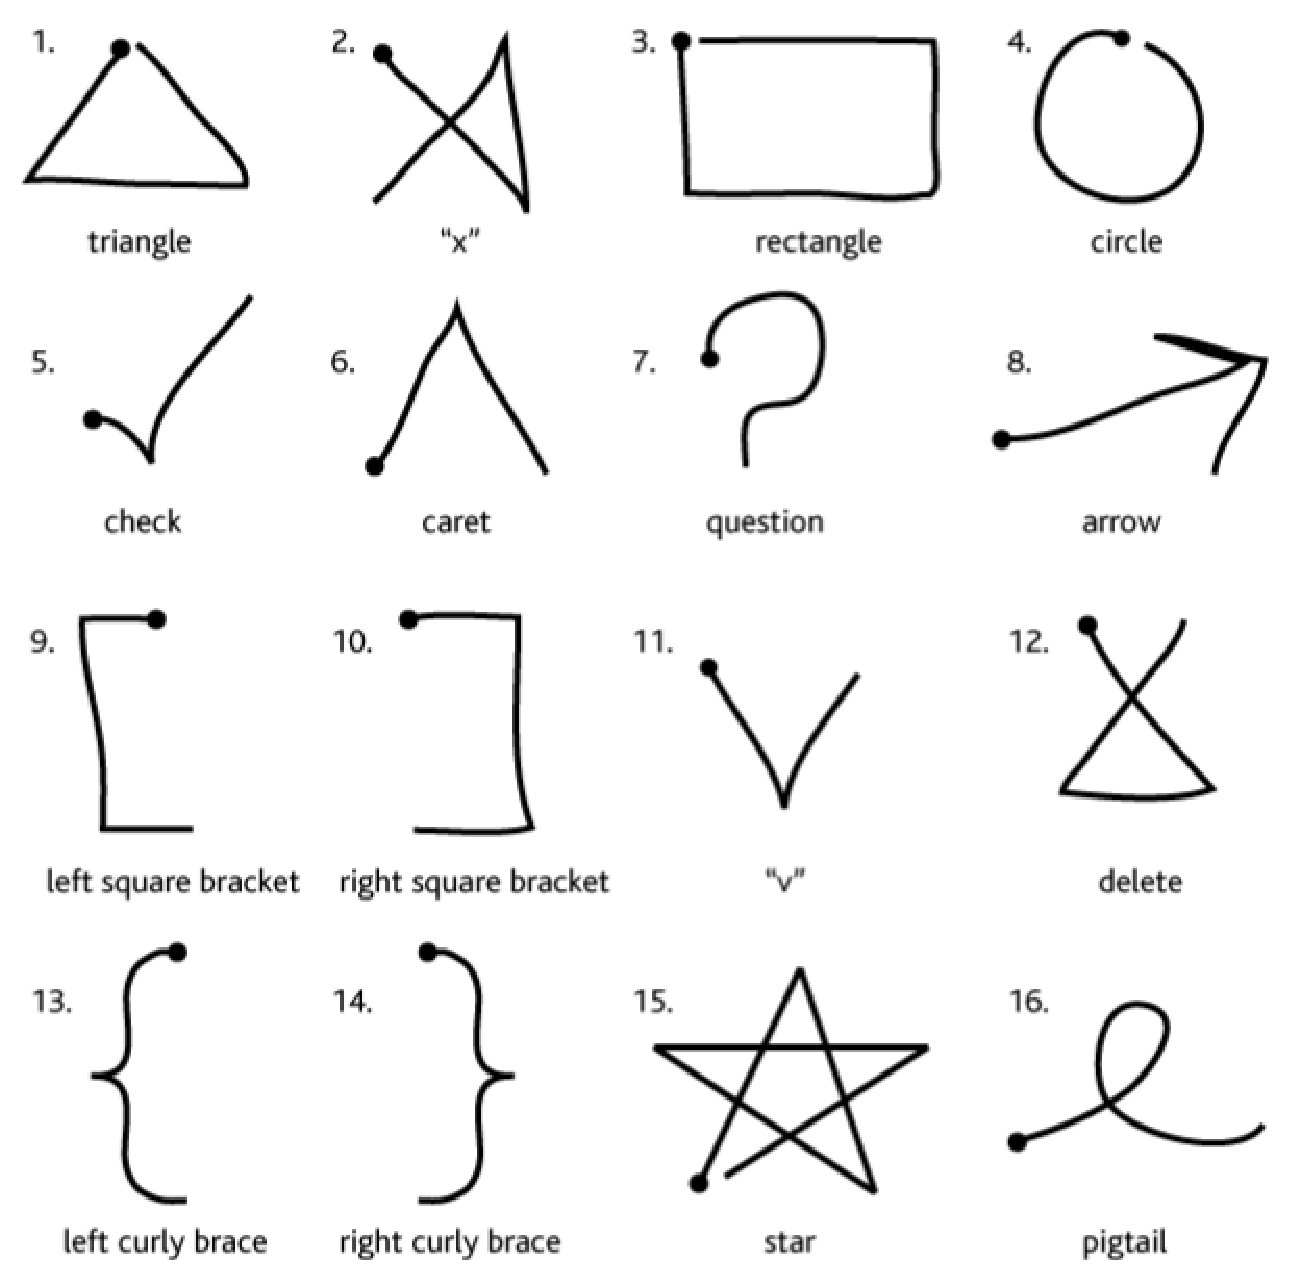
\includegraphics[width=0.4\columnwidth]{img/stroke_1.eps}
\caption{\$1において用いられる,スマートフォンやタブレット端末などのタッチパネルへの手書き入力やペン入力において一般的に良く用いられる,単一ストロークからなる手書きジェスチャの例,黒い点は手書きジェスチャの書き始めを示す.}
\label{fig:stroke_1}
\end{figure}

\section{被験者}
被験者は普段からスマートフォンを使用している男性6名である.年齢は21〜27歳~(平均23.8歳)であり,全員右利きであった.6名の被験者の中には大学院にてコンピュータサイエンスを専攻している人が4名存在し,残りの2名は,大学にて社会工学を専攻している男性と,エンジニアとして働いている男性であった.被験者は全員日頃からスマートフォンを使用していた.

%\section{調査に用いた機器}
%実験には,入力端末であるスマートフォンとしてiPhone5を用い,実験における入力領域は1.94'' × 3.18''であり,解像度は640 × 1036である~(図\ref{{fig:screenshot}}).

 %\begin{figure}[!h]
%\centering
%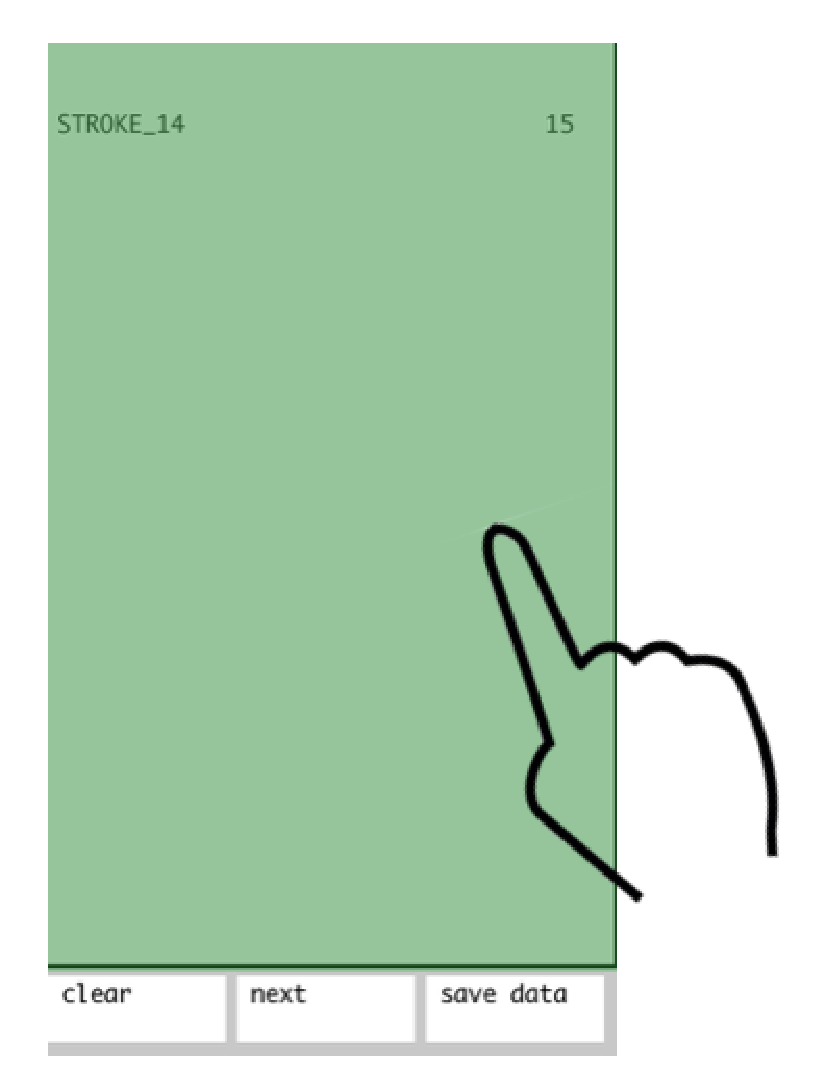
\includegraphics[width=0.4\columnwidth]{img/screenshot.eps}
%\caption{The screen shot on the smartphone. The green area is the input area}
%\label{fig:screenshot}
%\end{figure}

\section{調査手順}
%教示を詳しく書く
%使いたいジェスチャを入力することを示す
我々はまず,被験者に調査の目的を説明した.
その後,普段スマートフォンを利用する場面,およびスマートフォンを入力デバイスとしPCを操作する場面を想定した時,どのようなアプリケーションに対し,どのような手書きジェスチャを入力として用いたいかを20以上考えるよう指示し,自身のスマートフォンに対し実際に入力しながら考えるよう指示した.
%図\ref{fig:screenshot}における緑色の領域部分にジェスチャを入力するよう指示した.
その際,ジェスチャを入力する姿勢は次の3つの姿勢~(姿勢1,姿勢2,姿勢3)のうちのいずれかになるように指示した.
%から,実際に自分がそのジェスチャを入力として用いるときに入力する姿勢として各ジェスチャに対して1つ選んでもらった.
\begin{enumerate}
\item 机にスマートフォンをおいて,利き手の人差し指によって入力する.
\item 利き手でスマートフォンを握りながら,同じ利き手の親指によって入力する.
\item 利き手とは反対の手でスマートフォンを握りながら,利き手の人差し指によって入力する.
\end{enumerate}
被験者には,全ての姿勢を座って入力するよう指示した.これは,既存の\$-Family Recognizerにおいて手書きジェスチャの評価実験を行う際に,手書きジェスチャを座って入力することに統一するケースが多かったからである.
また,入力ジェスチャは単一ストロークからなるよう指示した.

入力として用いたい手書きジェスチャを1つ考えるたびに,我々は付録Bに示す紙にそのジェスチャをボールペンによって書くよう指示した.
またそれに加え,そのジェスチャをどのアプリケーションに対して用いたいのかも同時に書くよう指示した.
%そのジェスチャを入力した姿勢~(1〜3),そのジェスチャをどのアプリケーションに対して用いたいのかも同時に書くよう指示した.


\section{調査結果}
6人の被験者から得られた手書きジェスチャの一覧は付録Bに記載されている.

これらの結果からわかることは,
例えば図\ref{user}において示されるように,音楽プレイヤにおいて,早送り,巻き戻し,音量の上げ下げ,といったような前後への移動や,値の上げ下げなど,対になるような操作に対して,向きや大きさの違いを用いて入力する要望があった.また,ブラウザにおいて,位置によって登録先のブックマークを変える,ページ内における表示位置をジェスチャの入力位置に対応させる,といったように,位置の違いを操作対象先の違いに割り当てたり,現在操作しているものの位置に対応付けるといった要望があることがわかった.

また,片手で操作する姿勢~(姿勢2)においては,複雑な手書きジェスチャを入力することが困難であるため,極力簡単なストロークを用い,かつ,大きさ,向き,位置の特徴量を利用して入力する要望があることも分かった~(図\ref{user}における音楽アプリケーションの音量の上げ下げなど).
%\TODO{ここら辺もうちょい詳しく書く?}

\begin{figure*} [t]
 \begin{center}
  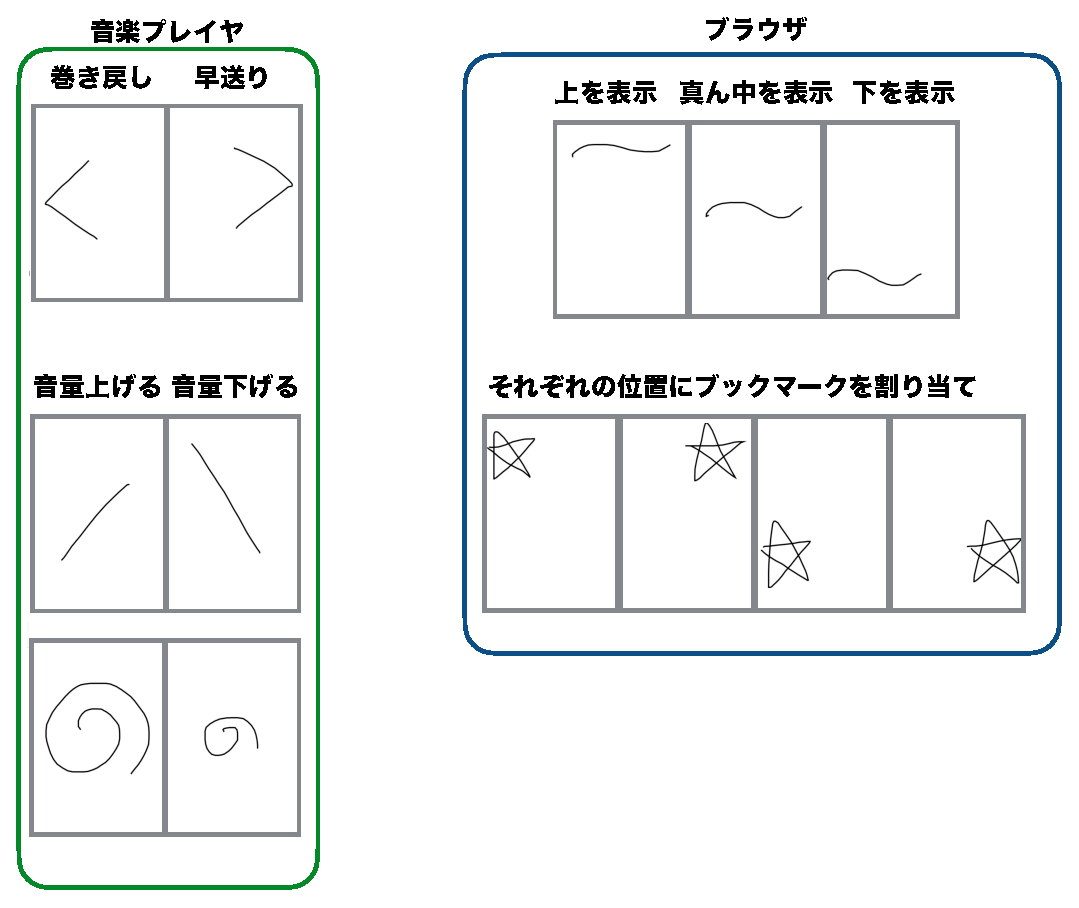
\includegraphics [width=0.8\columnwidth]{img/elicitation_example.eps}
  \caption{ユーザ調査において,ユーザが考案した手書きジェスチャとその利用例.}
  \label{user}
 \end{center}
\end{figure*}

ユーザ調査によって得られた手書きジェスチャは,重複しているジェスチャや\$1によって認識可能なジェス   チャも多く含まれていた.
本研究は,ジェスチャの形状や書き順は同じであるが,大きさ,向き,位置が異なる手書きジェスチャを識別することが目的であるため,
本研究における性能評価実験に用いる手書きジェスチャを,それぞれの被験者において,大きさ,向き,位置が異なる手書きジェスチャができるだけ多く含まれるように,かつジェスチャの数20以上となるように抜粋した~(図\ref{fig:elicetated_strokes}).

また,抜粋する際には,それぞれの手書きジェスチャに``STROKE\_1''のように番号を順に振り,それぞれの手書きジェスチャを入力する姿勢を,姿勢1〜姿勢3の中から1つ選んでもらい,手書きジェスチャとともにそれぞれ紙に記入した.

\$Vは,図\ref{fig:elicetated_strokes}に示すような,ジェスチャの形状や書き順は同じでも,大きさ,向き,位置に関して異なる手書きジェスチャを認識することが可能なアルゴリズムであり,今回調査を行った被験者の要望を満たすことのできる手書きジェスチャ認識アルゴリズムである.

\begin{figure*} [t]
 \begin{center}
  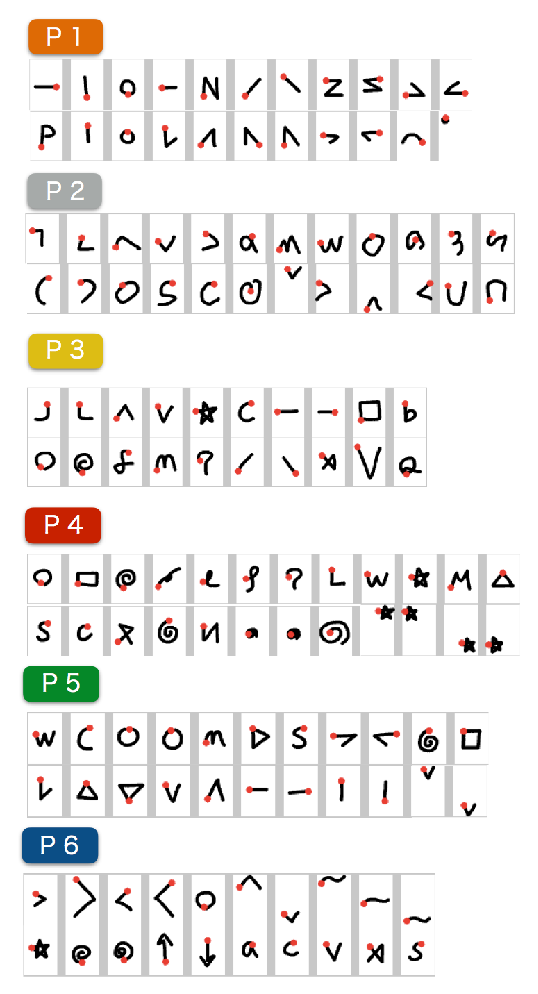
\includegraphics [width=0.65\columnwidth]{img/elicitated_strokes.eps}
  \caption{調査において6人の被験者~(P1〜P6)から得られた手書きジェスチャのうち,抜粋された手書きジェスチャ.}
  \label{fig:elicetated_strokes}
 \end{center}
\end{figure*}


%\$Vは,\$1にアルゴリズムを少し追加するだけで,\$1が示す認識率と認識速度を維持しつつ,図が示すような,ジェスチャの形状は同じでも,大きさ,向き,位置に関して異なるジェスチャ認識アルゴリズムである.






%$1
\chapter{\$1アルゴリズム}
\$Vは\$1の拡張であるため,本章において\$1アルゴリズムについて述べる.

\section{特徴}
ユーザが入力した手書きジェスチャは,図のように複数の点によって構成され,すでに登録された手書きジェスチャと,それぞれの点を比較することによって,どの手書きジェスチャと一致しているかが判別される.しかしながら,これらの手書きジェスチャを構成する複数の点は,入力に用いているハードウェアやソフトウェアに依存した速度によってサンプリングされる.それに加え,人間によって入力される手書きジェスチャはばらつきがあるため,入力される手書きジェスチャを構成する点の数は入力されるたびに異なる.
そのため,ユーザが入力した手書きジェスチャと,すでに登録された手書きジェスチャを比較するにあたり,手書きジェスチャを構成する点どうしを単純に比較することは困難であると言える.


例えば,図のような``pigtail''と``x''の手書きジェスチャのそれぞれのペアにおいて,手書きジェスチャの大きさや,手書きジェスチャを構成する点の数が異なる.この特徴は,手書きジェスチャ認識において双方を比較する上で,1つのハードルとなっている.
また,pigtailは回転することによってxと似た手書きジェスチャとなる.これらの問題に対処しつつ,単純なアルゴリズムを実現するために,以下のような基準に従うようなアルゴリズムの実現を目指した.

\begin{itemize}
\item ハードウェアやソフトウェアのセンシング及び入力する速度などによって変わるサンプリングされる点の数の違いに対してロバストであること.
\item 手書きジェスチャの大きさ,向き,位置の不変に関してオプショナルに設定可能であること.
\item 数学的な高度な知識やテクニックをを必要としないこと~(例えば,逆行列,微分,積分など)
\item 少ないコードによって実装できること.
\item 認識速度が速いこと.
\item ソフトウェア開発者やアプリケーションユーザが,独自に手書きジェスチャを定義できること.
\item N-best listに関して,高い識別能力を示すスコアを示すこと.
\item 図\ref{fig:stroke_1}のような単一ストロークからなる手書きジェスチャを認識するにあたり,HCI分野において多く用いられる既存の複雑な手書きジェスチャ認識アルゴリズムと比べても,高い認識率を示すこと.
\end{itemize}

ここで,N-best listとは,N個の学習データそれぞれに対する入力データとの類似度を降順に並べたものであり,N-best listの最高値と2番目の値の差が大きいほど,高い識別能力を示していると言える.

次に,これらの基準に従うような\$1のアルゴリズムを述べる.
アルゴリズムは大きく4つのステップから構成される.


\section{4つのステップ}
前節において述べた基準を満たすために,入力データ及び学習データは4つのステップを経た後に比較される.
4つのステップは,リサンプル,向きの正規化,大きさと位置の正規化,〜からなる.

\subsection{リサンプル}
前節において述べたように,手書きジェスチャを構成する点の数は,ハードウェアやソフトウェアのセンシング及び入力する速度などによって変わる.特に,入力速度の違いによる点の数の違いは顕著である.(図)

点の数が違うことにより,入力データと学習データの手書きジェスチャを構成する点を互いに比較することが困難となっている.そこで,図に示すようにN個の等間隔に並ぶ点にリサンプルすることとする.N個の点にリサンプルすることは,生のデータを扱うことと比べて正確なデータを扱っているとは言えず認識精度が落ちる可能性があるが,入力データと学習データ双方の手書きジェスチャの点の数が等しくなるため,容易に互いの対応する点を比較できる.

リサンプルすることは,既存の手書きジェスチャ認識アルゴリズムにおいても用いられている~\cite{Plamondon:2000:OOH:331097.331275, Tappert:1990:SAO:83123.83137, Kristensson:2004:SLV:1029632.1029640, Zhai:2003:SWS:642611.642630, Tappert:1982:CSR:1664966.1664979}.\$1はこれらのアルゴリズムを採用するとともに,これらのアルゴリズムとは違い向きに不変なアルゴリズムを提供する.また,手書きジェスチャを構成する点の数をリサンプルすることなく実行可能なDTWと比較している.

N個の等間隔に並ぶ点にリサンプルする方法を図に示す.
\TODO{リサンプルの仕方を図で説明}

また,32<N<256の時,N=64の時が最適であることがわかった.

\subsection{向きの正規化}
リサンプルされた手書きジェスチャの向きを``indicative angle''として定義する.indicative angleとは図のように,手書きジェスチャの書き始めの一番最初の点の座標,手書きジェスチャを構成する点全てによる中心座標,0度方向によって形成される角度である.そして,indicative angleの沿って,全てのジェスチャを回転させる.これにより,ジェスチャは向きに正規化される.


\subsection{大きさと位置の正規化}
向きによって正規化されたジェスチャの大きさを``boundingbox''として定義する.boundingboxとは図のように,ジェスチャに隣接するような矩形を示す.全てのジェスチャについて,boundingboxをある一定の大きさの矩形に正規化することによって,ジェスチャは大きさに正規化される.

大きさによって正規化されたジェスチャの位置をジェスチャを構成する全ての点による中心座標として定義する.全てのジェスチャについて(0, 0)へと移動させることによって,向きに正規化される.

\subsection{類似度を高くするための最適な角度}
リサンプルされた2つの手書きジェスチャ構成する点を1つずつ対応する点どうし比較するにあたり,1度ずつ手書きジェスチャを回転させながら,最も類似度が高くなるような角度を見つけた上で,類似度を算出する方法~\cite{Kara:2005:ITS:1652319.1652712}は認識のために膨大な時間を要することになる.学習データの数が全て含めて30くらいであればそのような方法でも十分な速度によって認識することが可能であるが,\$1は黄金分割探索~\cite{Press:1992:NRC:148286}を用いる.
黄金分割探索とは,単峰関数~(極値が1つしかない関数)において,極値を求めるための方法~(局所探索法)のうち効率的な方法の1つであり,極値が存在することが自明な範囲において極値を逐次的に求める方法である.

例えば図のように,f(x)の関数があり,極小値f(x')を求める時に,x1とx3の間に極値が存在することが自明な時に,その範囲内に存在するf(x2)を求める.この時x2は(x2 - x1) : (x3 - x2)が黄金比~(\TODO{黄金比入れる})となるように設定する.これが黄金分割探索と言われる所以であり,常に3点~(この場合x1, x2, x3)が存在する.その後広い区間~(この場合x2とx3の間)において,同様に黄金比によって分割し新たなf(x4)を得る.この時,f(x4a)ならば,極小値はx1とx4の間に存在するため,新たな3点はx1, x2, x4となる.f(x4b)ならば,極小値はx2とx3の間に存在するため,新たな3点はx2, x4, x3となる.このように,極小値が存在する範囲を徐々に狭めていくことによって,効率よく極小値を求めることができる.

\$1の場合,480個の手書きジェスチャにおいて,+-45度の範囲において極小値が存在することが発見され,極小値が存在する範囲が2度になるまで黄金分割探索を行う.この時,入力データに類似する学習データが存在する場合あるいはしない場合においても,10ステップ後には極小値が求められることが発見された.

局所探索法の1つである山登り法(引用)を黄金分割探索の代わりに用いる場合,480個の手書きジェスチャにおいて,類似するジェスチャの場合およそ7.2ステップ後に極小値を求めることができるが,類似するジェスチャが存在しない場合はおよそ53.5ステップ後に極小値が求められる.つまり学習データが10ずつ存在する16種類の手書きジェスチャ=160において,黄金分割探索は160\time10 = 1600ステップ必要であるのに対し,山登り法は7.2\time10 + 53.5\time150 = 8097ステップ必要であり,およそ80.2\%もの計算量の節約となっている.

このように,類似度を高くするための最適な角度を黄金分割探索によって効率的に求めることによって,認識速度の向上を実現している.

以上の4ステップをまとめ,入力データと学習データそれぞれを比較するまでの過程を図\ref{fig:algorithm_1}に示す.
\begin{figure} [!h]
\centering
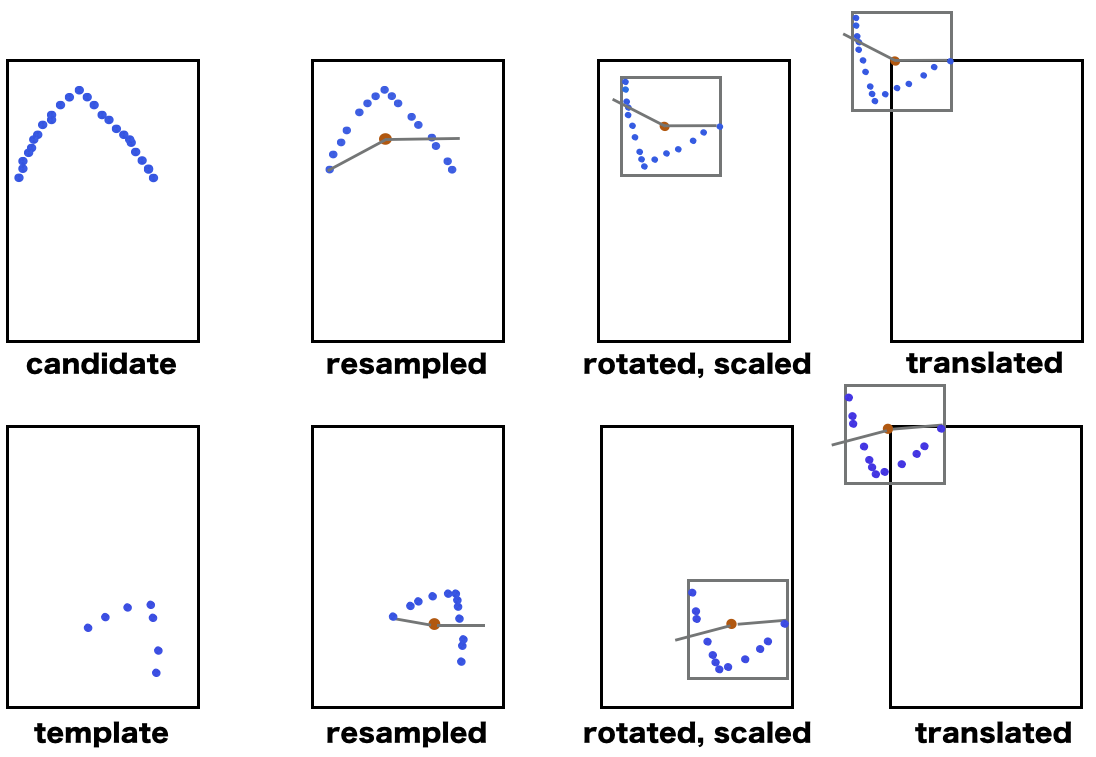
\includegraphics [width=0.8\columnwidth]{img/algorithm_1.eps}
\caption{Each step in the \$1 algorithm process}
\label{fig:algorithm_1}
\end{figure}

\subsection{類似度計算}
前節までの4ステップによって得られた入力データと学習データの最終的な類似度計算は式~(1)及び式~(2)によって表される.
\TODO{式を載せる}
ここで〜\TODO{式の説明}

\section{リミテーション}
\$1は,手書きジェスチャを,大きさ,向き,位置に正規化することによってアルゴリズム全体を簡潔化したり,それぞれについてロバストな認識を可能にし認識率の向上を実現した.しかしながら,このことが原因により,幾つかのリミテーションが存在する.

\begin{itemize}
\item 手書きジェスチャを大きさ,向き,位置によって識別しない.
\item 直線のような1次元の手書きジェスチャを認識することができない.
\item 手書きジェスチャを入力する速度による識別ができない.
\end{itemize}


「手書きジェスチャを大きさ,向き,位置によって識別しない」ことに関しては,それぞれについて正規化しないようにアルゴリズムを変えることによって識別することが可能となる.しかしながら,正規化しないことにより,正規化しないものに関してはロバスト性が低下するため,結果的に認識率の低下を招く恐れがある.

「直線のような1次元の手書きジェスチャを認識することができない」ことに関しては,向き,大きさに関して正規化した際に図のようになるためである.

「手書きジェスチャを入力する速度による識別ができない」ことに関しては,入力速度の要素を特徴量として用いることによって識別可能となる.例えば,Rubine~\cite{Rubine:1991:SGE:122718.122753}のような特徴量ベースの認識は,速度を特徴量として用いている.このように認識に用いる特徴量が複数存在する場合,用いる特徴量を適切に選択できれば,つまり,認識に本当に必要な特徴量のみを用いて,認識には必要のない特徴量を選択できれば,認識率の高い手書きジェスチャ認識アルゴリズムとなる.しかしながら,一般的に手書きジェスチャ認識アルゴリズムに関する深い知識がない限り,そのような適切な選択は困難である.\$1は,識別可能な特徴量が少ないが,そのようなわずらわしさを一切省いたアルゴリズムとなっている.





%$V
\chapter{\SysName アルゴリズム}
本章にて,\$1を拡張した\$Vアルゴリズムを述べる.

\section{\$Vアルゴリズムが目指す特徴}
\$Vアルゴリズムが目指す特徴を以下に示す.
\begin{itemize}
\item \$1の特徴を維持すること.つまり,
\begin{itemize}
\item ハードウェアやソフトウェアのセンシング及び入力する速度などによって変わるサンプリングされる点の数の違いに対してロバストであること.
%\item 手書きジェスチャの大きさ,向き,位置の不変に関してオプショナルに設定可能であること.
\item 数学的な高度な知識やテクニックをを必要としないこと~(例えば,逆行列,微分,積分など)
\item 少ないコードによって実装できること.
\item 認識速度が速いこと.
\item ソフトウェア開発者やアプリケーションユーザが,独自に手書きジェスチャを定義できること.
\item N-best listに関して,高い識別能力を示すスコアを示すこと.
\item 図\ref{fig:stroke_1}のような単一ストロークからなる手書きジェスチャを認識するにあたり,HCI分野において多く用いられる既存の複雑な手書きジェスチャ認識アルゴリズムと比べても,高い認識率を示すこと.
\end{itemize}
\item 前項目を満たした上で,形状や書き順が同じ手書きジェスチャを大きさ,向き,位置に関して識別可能にすること.
\end{itemize}

これまで述べてきたように,一般的に,特徴量を不変にすることによってその特徴量についてロバスト性が向上する.しかしながら,不変にしない場合,つまり,認識に用いる特徴量として扱う場合,ロバスト性が低下し,結果的に認識率の低下を招く恐れがある.つまり,\$1アルゴリズムを踏襲した上で,大きさ,向き,位置を特徴量として用い,それらに関して識別可能にするということは,\$1と比べて,認識率が低下すると言える.
以上を踏まえ,\$1と比べて,認識率や認識速度が著しく低下することなく,図\ref{fig:examples_V}のような,手書きジェスチャの形状と書き順は同じでも,大きさ,向き,位置が異なるジェスチャを識別するアルゴリズムを実現することが\$Vの目指すところである.

\section{\$Vアルゴリズムのアイディア}
本節にて,\$Vアルゴリズムのアイディアを述べる.

まず,形状や書き順が同じ手書きジェスチャを大きさ,向き,位置に関して識別可能にする方法を述べる.次に,\$1において認識できなかった1次元の手書きジェスチャを認識する方法を述べる.そして,\$Vアルゴリズムの最大の特徴である,学習データの保持の方法を述べる.

\subsection{大きさ,向き,位置に関して識別可能にする方法}
\$1アルゴリズムを活用し,ジェスチャを大きさ,向き,位置によって識別可能にするための方法として以下の2つが考えられる.
\begin{enumerate}
\item 単純にリサンプリングした点のみによって判別する~(正規化しない).
\item 正規化した上で,それぞれを特徴量として用いる.
\end{enumerate}
1. の場合,リサンプリングしただけの実質生データのまま比較するため,大きさ,向き,位置によって識別可能となる.しかしながら,手書きジェスチャの場合,アプリケーションユーザの入力は毎度微妙に異なることが予想される.そのため,類似したジェスチャにおいても,類似度が低くなり,ロバスト性が低下する恐れがあるとともに,認識されたか否かを判別するための類似度の閾値の設定が困難になることが予想される.
2. の場合,ジェスチャを正規化するためロバスト性は維持され,その上で,大きさ,向き,位置を特徴量として用いるため,1. の場合と比べて,類似度が低くなりづらくなると予想される.
そこで,\$Vは2. の方法を用いることとする.

\subsection{1次元の手書きジェスチャを認識する方法}
\$Vは\$1とは異なり,1次元の手書きジェスチャを認識できるようにした.これは\$N\cite{Anthony:2010:LMR:1839214.1839258}において実装されているため,その手法を用いる.
具体的には,\$1において大きさを正規化する際に用いられる,手書きジェスチャに隣接する矩形の縦の長さが横の長さに対し~(あるいはその逆が) 0.3未満の長さであれば,その手書きジェスチャは1次元の手書きジェスチャであるとみなし,大きさに正規化しない.これにより,1次元の手書きジェスチャを認識することが可能となる.

\subsection{学習データの保持の方法}
\$Vは学習データの保持の方法において特徴がある.

\$Vは学習データが追加されるたびに,ジェスチャの形状と書き順が同じ学習データを同じグループに分類する.ここでは形状と書き順が同じジェスチャを識別可能な\$1アルゴリズムを用いている.この形状と書き順に従って分類されたジェスチャを``ジェスチャグループ''と名付ける.ジェスチャグループの例を図\ref{fig:gesture_group}に示す~(あるいは図\ref{fig:examples_V}もジェスチャグループの例である).

\begin{figure} [h!]
	\begin{center}
		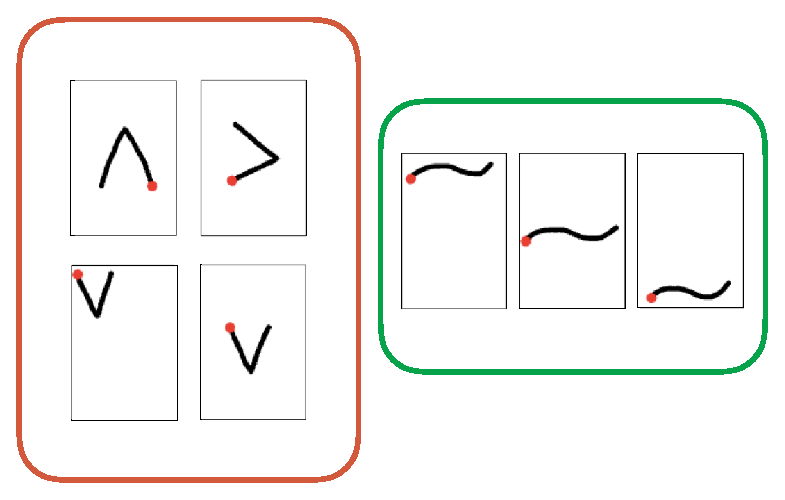
\includegraphics [width=0.7\hsize ]{img/gesture_group.eps}
	\end{center}
	\caption{形状と書き順が同じ手書きジェスチャの学習データが集まった,ジェスチャグループの例}
	\label{fig:gesture_group}
\end{figure}

このようにジェスチャグループを作成する理由は2つある.
\begin{itemize}
\item 認識速度の低下を防ぐため.
\item 認識率の低下を防ぐため.
\end{itemize}
それぞれについて理由を述べる.


\subsubsection{ジェスチャグループの作成が認識速度の低下を抑える理由}

大きさ,向き,位置を特徴量として認識に用いる場合,それぞれについての類似度計算を行うこととなる.これを全てのジェスチャについて行った場合,認識速度が低下する要因となる.
\$Vの目的は,ジェスチャの形状と書き順が同じであるが,大きさ,向き,位置に関して識別可能にすることである.そこで,形状と書き順が同じジェスチャが集まったジェスチャグループを作成し,入力データと学習データを比較した時に,形状と書き順が同じであったジェスチャグループ内に存在する学習データのみに対し,大きさ,向き,位置の類似度計算をする~(図\ref{fig:speed_reason}).一般的に,認識速度は,認識に用いる特徴量を増やした場合,増やさない場合と比べて,学習データの数に比例してその差が大きくなるが,同一ジェスチャグループ内のみに対し認識に用いる特徴量を増やすことによって,全体的な認識速度の低下を防ぐことが可能となると考えた.以上を踏まえ我々は「ジェスチャグループを作成し,形状と書き順が同じであるジェスチャグループ内に存在する学習データのみに対し,大きさ,向き,位置の類似度計算をすると認識速度の低下を抑えることができる」という仮説を立てた.

\begin{figure} [h!]
	\begin{center}
		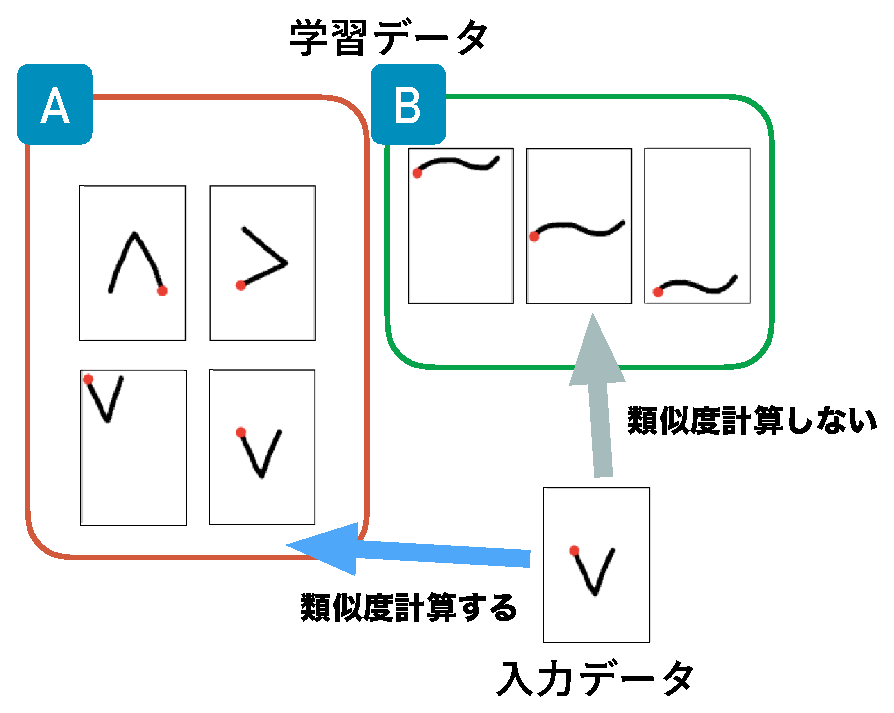
\includegraphics [width=0.6\hsize ]{img/speed_reason.eps}
	\end{center}
	\caption{同一ジェスチャグループ~(A)のみに対し,大きさ,向き,位置の類似度計算を行う.}
	\label{fig:speed_reason}
\end{figure}

\subsubsection{ジェスチャグループの作成が認識率の低下を抑える理由}

大きさ,向き,位置の特徴量を認識のために全てのジェスチャに対し用いた場合を考える.
例えば,図\ref{fig:cannot_recognized}Aの場合について考える.
入力データ~(図\ref{fig:cannot_recognized}A')が図\ref{fig:cannot_recognized}Aの右下のジェスチャと一致させようと入力されたとする.しかし,この2つのジェスチャは大きさが異なるため,大きさを認識のための特徴量として用いている限り類似度が低下し認識率が下がることが考えられる.また,これはロバスト性の低下につながる.

図\ref{fig:cannot_recognized}Bの場合について考える.
入力データ~(図\ref{fig:cannot_recognized}B')が図\ref{fig:cannot_recognized}Bの右のジェスチャと一致させようと入力されたとする.しかし,この2つのジェスチャは向きが異なるため,向きを認識のための特徴量として用いている限り類似度は低下し認識率が下がることが考えられる.また,これはロバスト性の低下につながる.

図\ref{fig:cannot_recognized}Cの場合について考える.
入力データ~(図\ref{fig:cannot_recognized}C')が図\ref{fig:cannot_recognized}Cのジェスチャと一致させようと入力されたとする.しかし,この2つのジェスチャは大きさ,向き,位置が異なるため,大きさ,向き,位置を認識のための特徴量として用いている限り類似度は低下し認識率が下がることが考えられる.また,これはロバスト性の低下につながる.

これまでに述べてきたが,大きさ,向き,位置を認識のための特徴量として新たに用いることによって,それぞれについてロバスト性が低下,つまり,認識率の低下を招く恐れがある.図\ref{fig:cannot_recognized}はその例である.

\begin{figure} [h!]
	\begin{center}
		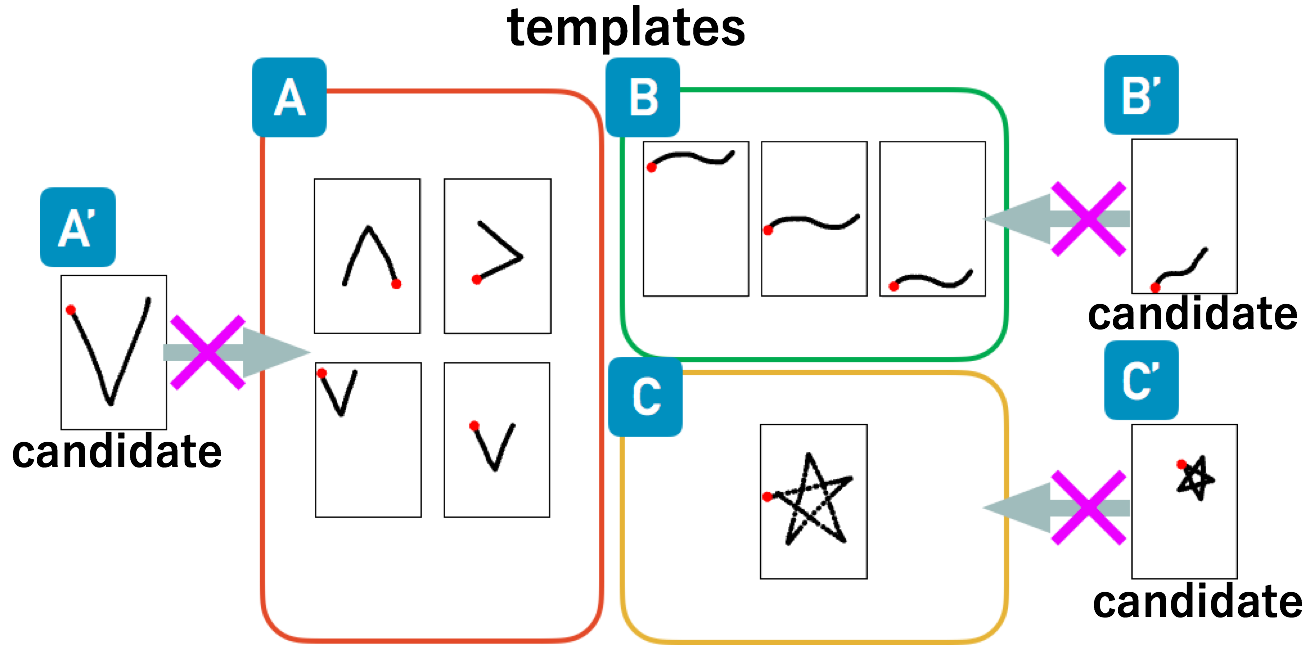
\includegraphics [width=0.8\hsize ]{img/cannot_recognized.eps}
	\end{center}
	\caption{大きさ,向き,位置を特徴量として認識のために用いた場合に,入力データと学習データが一致しない例}
	\label{fig:cannot_recognized}
\end{figure}

そのため,\$Vでは,大きさ,向き,位置を認識のための特徴量として単に用いるのではなく,
ジェスチャグループごとに,大きさ,向き,位置のうちどの特徴量を認識に用いるか選ぶ,つまり,識別するために必要な特徴量を選ぶ
という処理を施すことによってロバスト性を維持できる部分を維持する.これにより,認識率の低下を防ぐことが可能となると考えた.

\subsubsection{ジェスチャグループごとの特徴量の選定}
ジェスチャグループごとに,大きさ,向き,位置のうちどの特徴量を用いるかを選ぶための方法を述べる.

\$Vの目的は,ジェスチャの形状と書き順が同じであるが,大きさ,向き,位置に関して識別可能にすることである.つまり,同一ジェスチャグループにおいて,大きさ,向き,位置のいずれかあるいはすべてが異なるジェスチャを識別できれば良い.

ここで,図\ref{fig:cannot_recognized}Aの場合について考える.
図\ref{fig:cannot_recognized}Aのジェスチャグループには,ジェスチャの大きさはどの学習データも同じであるが,向きや位置が異なるジェスチャが存在している.つまり,これらを識別するためには,向き,位置を特徴量として認識に用いることが必要となる.反対に,大きさは特徴量として認識に用いる必要がない.

図\ref{fig:cannot_recognized}Bのジェスチャグループには,ジェスチャの大きさや向きはどの学習データも同じであるが,位置が異なるジェスチャが存在している.つまり,これらを識別するためには,位置を特徴量として認識に用いることが必要となる.大きさや向きは特徴量として認識に用いる必要がない.

図\ref{fig:cannot_recognized}Cのジェスチャグループには,1種類のジェスチャしか存在していない.つまり,識別のために大きさ,向き,位置全ての特徴量も認識に用いる必要がない.

このようにして,ジェスチャグループに存在する学習データの特徴によって,認識に用いる特徴量を選ぶ,つまり,ある特徴量については認識のために特徴量として用いないことによって,その特徴量について不変にし,ロバスト性を維持する.これにより認識率の低下を防ぐことが可能となる.

以上を踏まえ我々は,「同一ジェスチャグループ内において,他の学習データと類似している特徴量は,認識のための特徴量として用いなければ,認識率の低下を抑えることができる」という仮説を立てた.

\section{認識に用いる特徴量を選定した時の認識率と認識速度の実験}
5.2節までにおいて述べてきた,ジェスチャグループを作成し,形状と書き順が同じであるジェスチャグループ内に存在する学習データのみに対し,大きさ,向き,位置の類似度計算をすると認識速度の低下を抑えることができるという仮説と,
同一ジェスチャグループ内において,他の学習データと類似している特徴量は,認識のための特徴量として用いなければ,認識率の低下を抑えることができるという仮説を検証するための実験を行った.
本節にてまず,実験を行うにあたって,大きさ,向き,位置,それぞれの特徴量と類似度の定義,ジェスチャグループの作成方法,ジェスチャグループにおける認識に用いる特徴量の選定方法をそれぞれ具体的に述べてから,実験の内容を述べる.

\subsection{ジェスチャの特徴量と類似度の定義}
ジェスチャの大きさ,向き,位置を特徴量として用いた時の,それぞれの特徴量と類似度の定義を示す.

\subsubsection{大きさ}
ジェスチャを構成するストロークの点を内包するように隣接した矩形の面積をジェスチャの大きさとして定義する (図\ref{fig:v_size}).
そして,2つのジェスチャの類似度$S_\textit{s}$を式5.1によって定義する.

\begin{figure} [h!]
	\begin{center}
		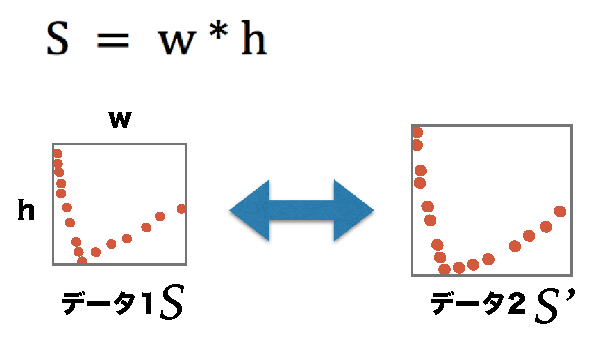
\includegraphics [width=0.45\hsize ]{img/v_size.eps}
	\end{center}
	\caption{大きさの定義}
	\label{fig:v_size}
\end{figure}

\begin{equation}
S_\textit{s} = \left \{
\begin{array}{l}
\frac{S'}{S} (S>S') \\\\
\frac{S}{S'} (S'>S')
\end{array}
\right.
\end{equation}
ここで,Sはデータ1の矩形の面積,S'はデータ2の矩形の面積である.

\subsubsection{向き}
ジェスチャを構成するストロークの始めの点の座標,全サンプル点の中心座標,その中心座標から右横に延長した線(0度)によって形成させる角度すなわち indicative angle をジェスチャの向きとして定義する(図\ref{fig:v_orientation}).
そして,2つのジェスチャの類似度$S_\textit{o}$を式5.2によって定義する.

\begin{figure} [h!]
	\begin{center}
		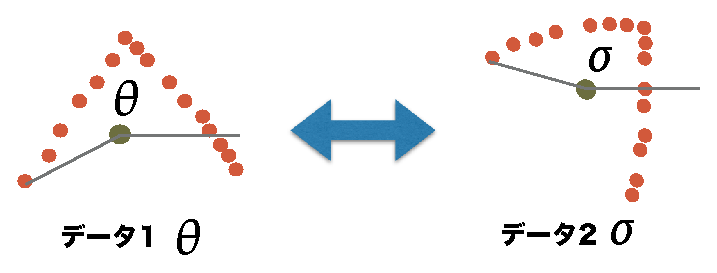
\includegraphics [width=0.6\hsize ]{img/v_orientation.eps}
	\end{center}
	\caption{向きの定義}
	\label{fig:v_orientation}
\end{figure}

\begin{equation}
S_\textit{o} = 1 - \frac{|\theta - \sigma|}{\pi}
\end{equation}
ここで,$\theta$はデータ1の向き,$\sigma$はデータ2の向きである.


\subsubsection{位置}
ジェスチャを構成するストロークのすべての点の中心座標をジェスチャの位置として定義する(図\ref{fig:v_position}).
そして,2つのジェスチャの類似度$S{\scriptsize p}$を式5.3によって定義する.

\begin{figure} [h!]
	\begin{center}
		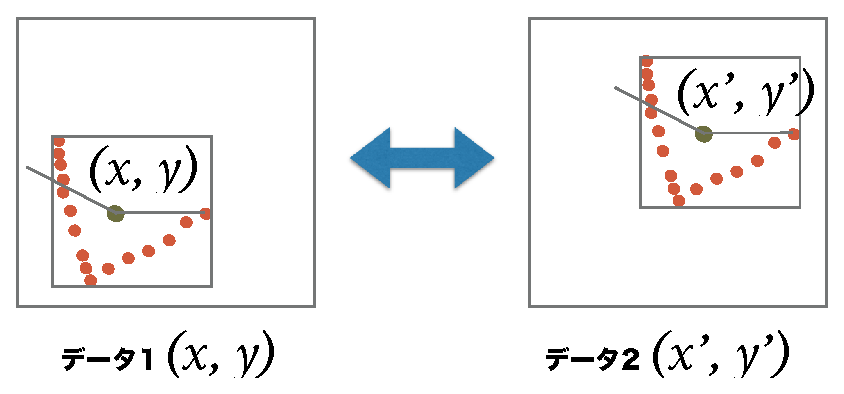
\includegraphics [width=0.6\hsize ]{img/v_position.eps}
	\end{center}
	\caption{位置の定義}
	\label{fig:v_position}
\end{figure}


\begin{equation}
S_\textit{p} = 1 - \frac{\sqrt{(x - x')^2 + (y - y')^2}}{\sqrt{W\!idt\!h^2 * H\!ei\!ght^2}}
\end{equation}
ここで,$(x, y)$はデータ1の位置,$(x', y')$はデータ2の位置であり,$Width$は入力領域全体の横,$Height$は縦の長さである.

また,大きさ,向き,位置の特徴量はそれぞれ,\$1において計算されているものであるため,再利用することによって計算量の増加を抑える.

\subsection{ジェスチャグループの作成方法}
ジェスチャの形状と書き順が同じ学習データが集まったグループである,ジェスチャグループを作成するための手順を以下に示す.
まず,学習データが新たに追加される場面を考える.
\begin{enumerate}
\renewcommand{\labelenumi}{\Alph{enumi}.}
\item 同じ名前の学習データが存在する場合~(図\ref{fig:same_gesture})

%同じジェスチャとして管理される.
新たに追加された学習データは同じ名前の学習データと一緒に保管される.この時,その名前を持つ学習データの,大きさ,向き,位置の特徴量は,それぞれの特徴量の算術平均によって表される~(図\ref{fig:same_gesture}).

\begin{figure} [h!]
	\begin{center}
		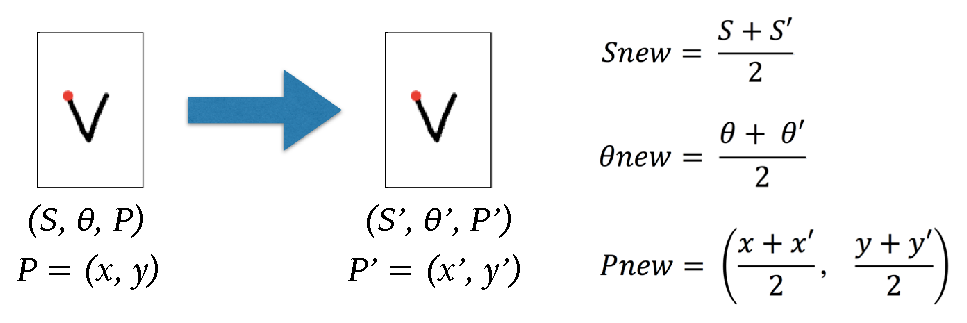
\includegraphics [width=0.9\hsize ]{img/same_gesture.eps}
	\end{center}
	\caption{同じ名前の学習データが追加された時に,それぞれの大きさ,向き,位置の特徴量を(S, $\theta$, P),(S', $\theta$', P')とした時の,そのジェスチャの新たな特徴量の求め方.}
	\label{fig:same_gesture}
\end{figure}

ここで,図\ref{fig:same_gesture}において,$S_\textit{new}$,$\theta_\textit{new}$,$P_\textit{new}$は,同じ名前の学習データにおける,大きさ,向き,位置の特徴量を示している.

 
\item 同じ名前の学習データが存在しない場合

\$1アルゴリズムを用いることによりジェスチャの形状と書き順を判断し,

\begin{enumerate}
\renewcommand{\labelenumi}{\alph{enumi}.}

\item 同じ形状と書き順のジェスチャグループが存在しない場合~(図\ref{fig:make_gesture_group}C)
 
%別の形状のジェスチャのグループとして管理される
新たに追加された学習データは新しい,ジェスチャグループとして保管される.
   
\item 同じ形状と書き順のジェスチャグループが存在する場合~(図\ref{fig:make_gesture_group}A)

%次節にて詳細を述べる.
そのジェスチャグループに保管される.

\end{enumerate}
\end{enumerate}

\begin{figure} [h!]
	\begin{center}
		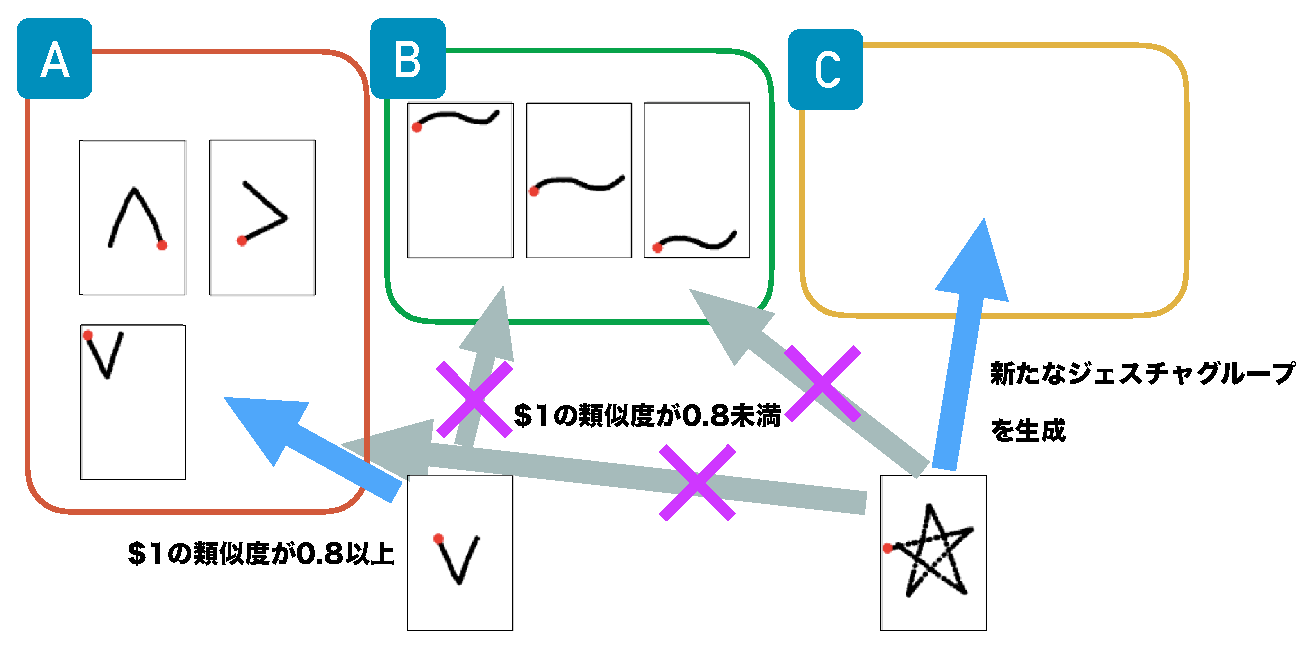
\includegraphics [width=0.9\hsize ]{img/make_gesture_group.eps}
	\end{center}
	\caption{学習データを新たに追加する場面の例}
	\label{fig:make_gesture_group}
\end{figure}

ここで,新たに追加された学習データが,既存のジェスチャグループに対し形状と書き順が同じかどうかを判別する方法は,既存のジェスチャグループ内の学習データ1つ1つと比較することによって行う.今回は\$1による類似度が0.8を超えたときに,形状と書き順が同じであると判断した.これは\$1アルゴリズムにて,類似度のN-best Listの1番目と2番目のスコアの差が0.2以上であることを利用している.
%ここで,類似度のN-best Listとは,N 個の学習データそれぞれに対するテストデータとの類似度を降順に並べたもの,1番目と2番目の差が大きいほど識別性能が高いことを示す.
もし1つでも形状と書き順が同じジェスチャが存在すれば,そのジェスチャが存在するジェスチャグループに保管される.なお,保管候補のジェスチャグループが複数存在する場合は,最も類似度が高かったジェスチャが存在するジェスチャグループに保管される.


\subsection{ジェスチャグループにおける認識に用いる特徴量の選定方法}
我々は,同一ジェスチャグループ内において,他の学習データと類似している特徴量は,認識のための特徴量として用いなければ,認識率の低下を防ぐことができるという仮説を立てた.
ここで,同一ジェスチャグループ内における他の学習データとの類似度を``ジェスチャグループの学習データ間の類似度''とし,その定義を以下のように定める.

まず,同一ジェスチャグループ内において,学習データを2つずつ抽出し,それぞれのペアについて学習データどうしの大きさ,向き,位置の類似度を式5.1〜式5.3を用いて求める.そして,各ペアにおける類似度を比較した時に,それぞれの特徴量について,最小となった類似度を,その形状グループの学習データ間のそれぞれの特徴量についての類似度とする.

例えば,図\ref{fig:group_similarity}左に示すジェスチャグループの場合,同一ジェスチャグループ内に4つの学習データが存在する.そのため,2つずつ抽出した場合の学習データの組み合わせは${\scriptsize 4}C{\scriptsize 2}=6$通り存在する~(図\ref{fig:group_similarity}右).それぞれのペアについて,学習データどうしの大きさ,向き,位置の類似度はそれぞれのペアにおいて図\ref{fig:group_similarity}右に示されている.この時それぞれの類似度の最小値は,大きさは0.8,向きは0.1,位置は0.4となるため,このジェスチャグループの学習データ間の類似度は~(大きさ,向き,位置) =~(0.8, 0.1, 0.4)となる~(図\ref{fig:group_similarity}左).
ここで,類似度の最小値を用いる理由は,類似度が小さいということは,その特徴量に関して類似していないことを示し,類似していない学習データの組み合わせが1つでも存在すれば,その特徴量について識別するために,認識のための特徴量として用いる必要があると考えたからである.

\begin{figure} [h!]
	\begin{center}
		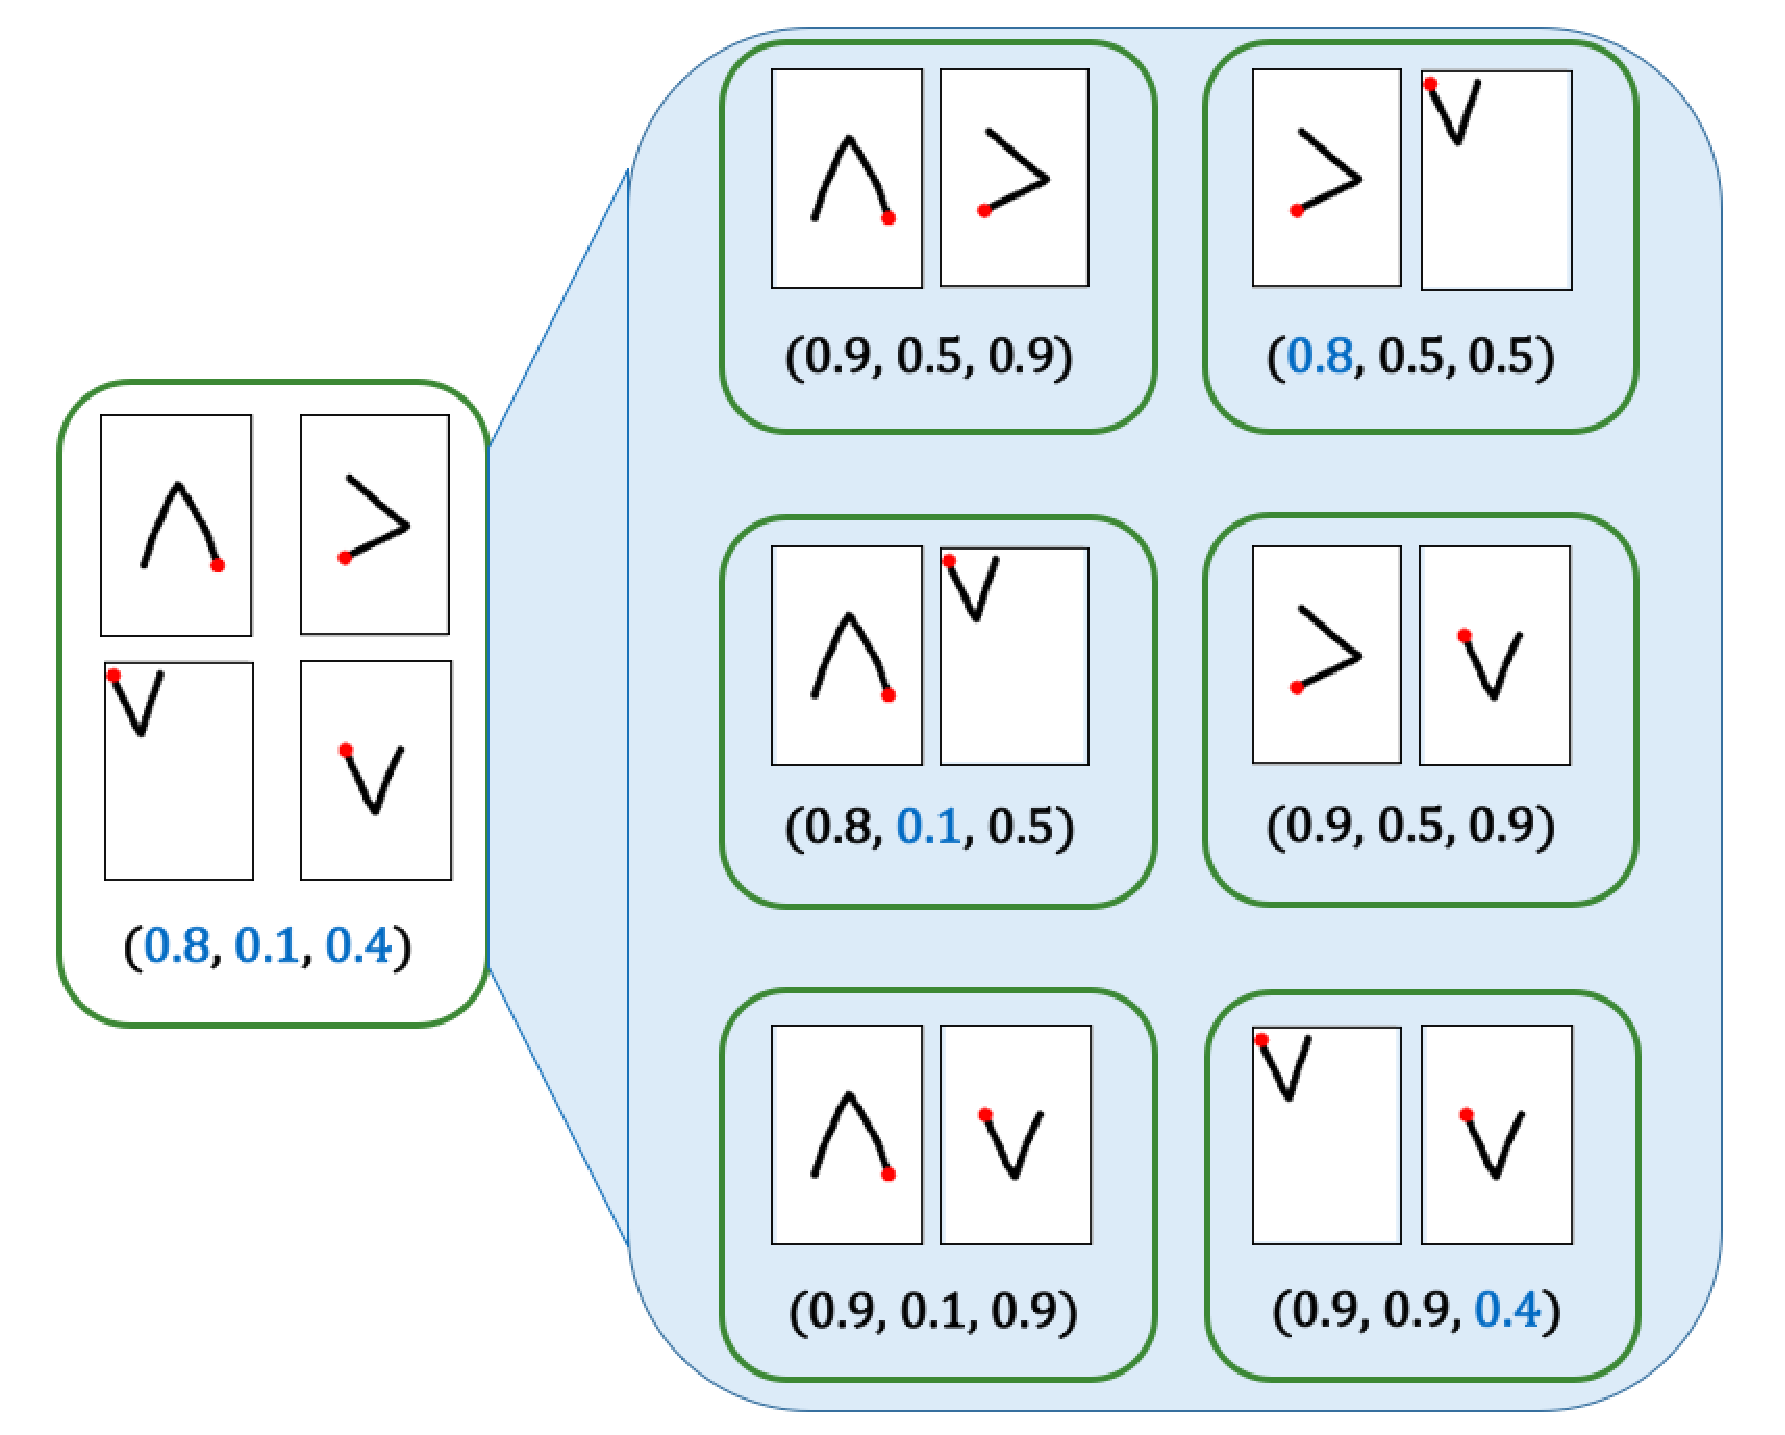
\includegraphics [width=0.8\hsize ]{img/group_similarity.eps}
	\end{center}
	\caption{ジェスチャグループの学習データ間の類似度を求める方法,この場合,~(大きさ,向き,位置) =~(0.8, 0.1, 0.4)となる.}
	\label{fig:group_similarity}
\end{figure}

以上のようにして得られたジェスチャグループの学習データ間の類似度を用いて,そのジェスチャグループが認識に用いる特徴量を選定する.本実験においては,類似度が0.2を下回った特徴量を,認識に用いる特徴量として選定した.


\subsection{ジェスチャの認識方法}
入力データの認識方法の手順は2つである.
\begin{enumerate}
\item \$1アルゴリズムを用いることにより,どのジェスチャグループに属するか判別する.この時,学習データを追加する時と同様,ジェスチャグループ内のすべての学習データに対し類似度を求め,0.8を超えた場合あるいは,0.8を超えるジェスチャが複数存在する場合は,最も類似度が高いジェスチャが存在するジェスチャグループに属すると判別する.
\item 1.によって判別されたジェスチャグループ内において,どのジェスチャと最も類似しているかを判別する.
\end{enumerate}
2. において,類似度$S_\textit{final}$は以下の式によって求められる.
\begin{equation}
S_\textit{final} = \frac{S_\textit{cs} \times α_\textit{s} + S_\textit{co} \times α_\textit{o} + S_\textit{cp} \times α_\textit{p}}{n}
\end{equation}

\begin{equation}
α_\textit{s}= \left \{
\begin{array}{l}
1 (S_\textit{ts}<0.2) \\\\
0 (else)
\end{array}
\right.
\end{equation}

\begin{equation}
α_\textit{o}= \left \{
\begin{array}{l}
1 (S_\textit{to}<0.2) \\\\
0 (else)
\end{array}
\right.
\end{equation}

\begin{equation}
α_\textit{p} = \left \{
\begin{array}{l}
1 (S_\textit{tp}<0.2) \\\\
0 (else)
\end{array}
\right.
\end{equation}

ここで,$S_\textit{cs}$は入力データと学習データの大きさの類似度,$S_\textit{co}$はジェスチャグループの入力データと学習データの向きの類似度,$S_\textit{cp}$はジェスチャグループの入力データと学習データの位置の類似度を示しており,$S_\textit{ts}$はジェスチャグループの学習データ間の大きさの類似度,$S_\textit{to}$は学習データ間の向きの類似度,$S_\textit{tp}$は学習データ間の位置の類似度を示している.また,nは1となる$α_\textit{s}$,$α_\textit{o}$,$α_\textit{p}$の数であり,0 $\leq$ n $\leq$ 3を満たす正の整数である.なお,n = 0の時,$S_\textit{final}$は計算せず,手順1.において,最も類似度が高いジェスチャを一致するジェスチャとして判別する.

\subsection{被験者}
被験者は,第3章のユーザ調査において協力してもらった6名である~(男性6名,21〜27歳~(平均23.8歳),全員右利き).

\subsection{実験機器}
実験には,入力端末としてiPhone5を用い,実験における入力領域は1.94'' × 3.18''であり,解像度は640 × 1036である~(図\ref{fig:screenshot}における緑色の部分).

\begin{figure}[!h]
\centering
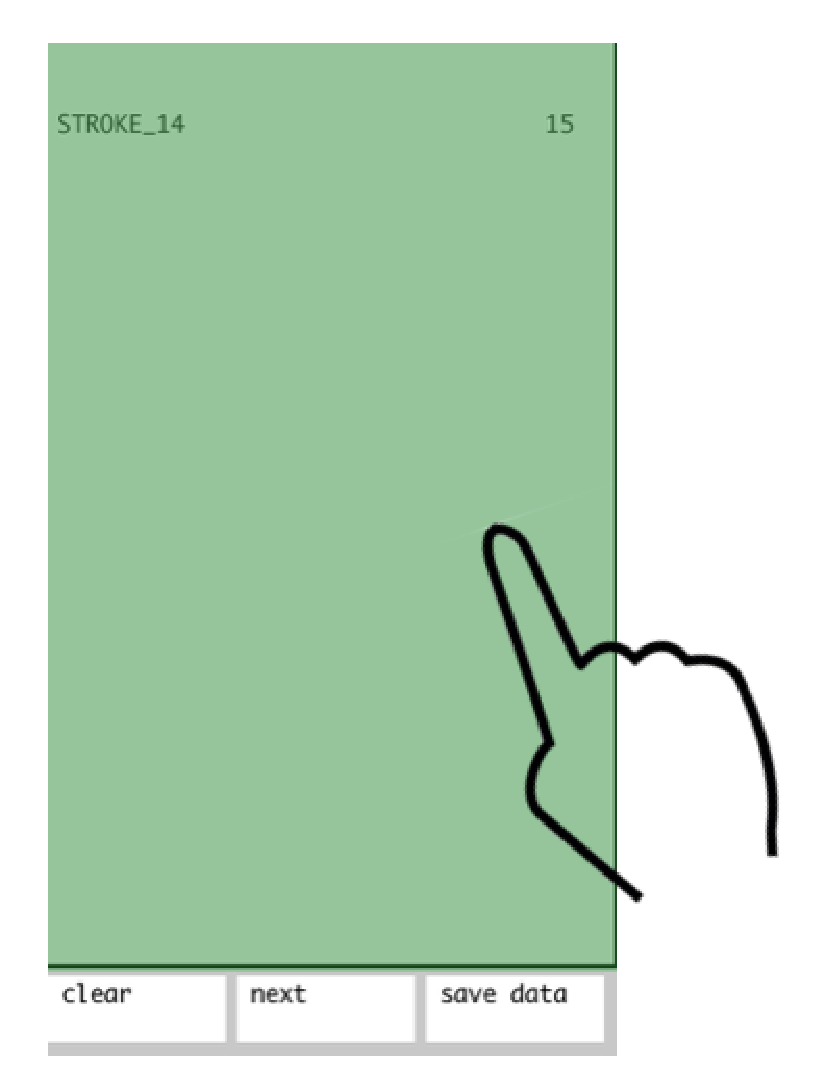
\includegraphics[width=0.4\columnwidth]{img/screenshot.eps}
\caption{実験に用いたスマートフォンのスクリーンショット.緑色のエリアはジェスチャが入力されるエリア.}
\label{fig:screenshot}
\end{figure}


\subsection{実験手順}
\subsubsection{ジェスチャの取得}
我々はまず,被験者に実験の目的を説明した.
その後,ユーザ調査において記入してもらった紙を見ながら,自身が入力したそれぞれのジェスチャを入力するよう指示した.
この,それぞれの被験者ごとのジェスチャを``ジェスチャセット''とする.
ジェスチャは図\ref{fig:screenshot}における緑色の領域部分にジェスチャを入力するよう指示した.
その際,そのジェスチャを入力するときの姿勢が紙に書かれているため,それに従い入力するよう指示した.
それぞれのジェスチャセットにおいて,ジェスチャには,ジェスチャ番号がSTROKE\_1のようにして割り振られており,図\ref{fig:screenshot}に示すように,画面左上に入力すべきジェスチャが表示される.
タスクの1試行は被験者が1つのジェスチャを入力するまでである.被験者はランダムに選択されたそれぞれのジェスチャを1回ずつ入力し,自身のジェスチャセットに含まれるジェスチャ全てを入力し,これを1セッションとした.これを10セッション行った.被験者によって入力すべきジェスチャの数は異なるが,いずれの被験者においても20以上のジェスチャを入力する(20〜24個のジェスチャ,平均22個).したがって,被験者は平均して計220試行~(22ジェスチャ $\times$ 10セッション)行った.
ジェスチャが思うように入力できなかった場合には,何度でも書き直し可能とした.

\subsubsection{認識率と認識速度の測定}
本実験において被験者は6人であるため,ジェスチャセットは6つ存在する.実験は各被験者が自身のジェスチャセットについてのみ行うためユーザ依存となる.それぞれのジェスチャは10個ずつあり,学習データをランダムにE個選んだ.その際のジェスチャグループの決め方と,ジェスチャグループの学習データ間の類似度の計算方法は,5.3.2節及び5.3.3節に示したとおりである.学習データを追加し終わった後,入力データを残りの10 - E個のジェスチャからランダムに1個選び,認識率と認識速度を測定した~(10分割交差検定).これをそれぞれのジェスチャにつき100回行った.本実験はE = 1〜5とした.また,認識率はジェスチャセットにおける認識率の100回平均を学習データごとに測定し,認識速度は,ジェスチャ1つを認識し終わるまでに要した時間について,ジェスチャセットに含まれる全ジェスチャの平均値の100回平均を測定し,テストに用いるジェスチャをランダムに選ぶ過程は含まれていない.

\subsubsection{N-best Listの1番目と2番目のスコアの差と類似度の測定}
認識率と認識速度に加え,類似度のN-best Listの1番目と2番目のスコアの差及びジェスチャが正しく認識された時の,類似度の測定も行う.ここで,類似度のN-best Listとは,N 個の学習データそれぞれに対するテストデータとの類似度を降順に並べたものであり,1番目と2番目のスコアの差が大きいほど識別性能が高いことを示す.また,本実験においては,正しく認識されたジェスチャの類似度の平均値の100回平均,正しく認識されたジェスチャのうち,類似度が最も低かったジェスチャの100回平均も測定した.


\subsection{実験結果と考察}
それぞれの被験者ごとの認識率,認識速度,N-best Listの1番目と2番目のスコアの差,ジェスチャが正しく認識された時の類似度,ジェスチャが正しく認識された時の類似度の最小値を示す.

本実験は,特徴量を選定する手法を用いた場合において,上記についてを測定することが目的であるが,
正規化せずにリサンプリングした点のみによってジェスチャを比較する手法及び,ジェスチャグループごとに特徴量を認識に用いるが選定しない手法,つまり,どのジェスチャグループに対しても大きさ,向き,位置の特徴量を類似度に用いる手法についても比較のために測定を行った.

\subsubsection{認識率}
図\ref{fig:rare_rec}に各手法ごとの認識率を示す.
特徴量を選定する手法及び特徴量を選定しない手法は,どの被験者のジェスチャセットにおいても80\%以上であり,認識率は高かった.
リサンプリングのみの場合は,ジェスチャセットによっては認識率は低かった.
また,リサンプリングのみの手法は,学習データの数に比例して認識率が高くなったが,特徴量を選定する手法及び特徴量を選定しない手法において,認識率は必ずしも学習データの数と認識率は比例しなかった.

これは,リサンプリングのみの手法は,学習データが増えるほど,入力データに類似する学習データが存在する可能性が高くなるが,特徴量を選定する手法及び特徴量を選定しない手法は,同じジェスチャの学習データを追加するたびに,大きさ,向き,位置それぞれの特徴量を算術平均するため,必ずしも入力データに類似する学習データが存在する可能性が高くなるとは言えないからである.

\begin{figure}[!h]
\centering
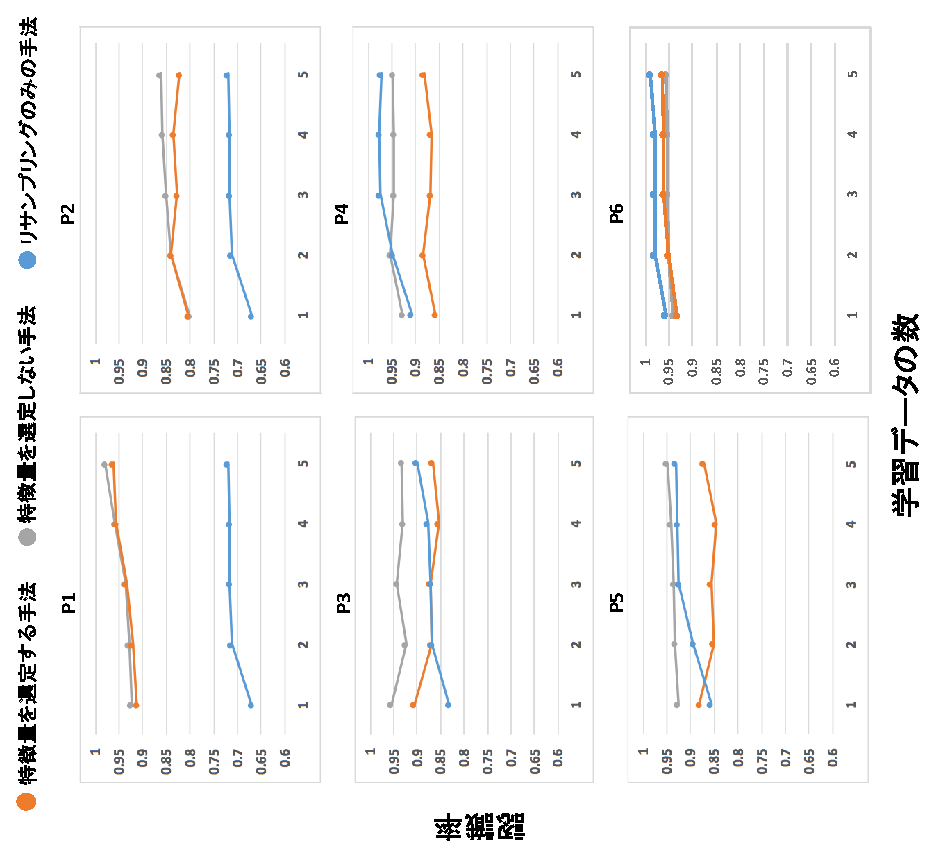
\includegraphics[width=0.9\columnwidth]{img/pre_rec.eps}
\caption{各手法における,被験者ごとの認識率の平均}
\label{fig:rare_rec}
\end{figure}

\subsubsection{認識速度}
図\ref{fig:rare_speed}に各手法ごとの認識速度を示す.
いずれの手法においても,認識速度はほとんど変わらなかった.リサンプリングのみの手法は,正規化処理を行わないため,最も認識速度は速くなった.特徴量を選定しない手法は,正規化したのち,特徴量を選定するための処理を行わないため次に認識速度が速くなった.特徴量を選定する手法は正規化に加え,特徴量を選定する処理を行う必要があるため最も認識速度が遅くなった.しかしながら,特徴量を選定する手法及び特徴量を選定しない手法の認識速度は,リサンプリングのみの手法と同程度であり,ェスチャグループ内に存在する学習データのみに対し,大きさ,向き,位置の類似度計算をすると認識速度の低下を抑えることができるという仮説は正しいと言える.
また,どの場合においても認識速度は学習データの数に比例して遅くなった.

\begin{figure}[!h]
\centering
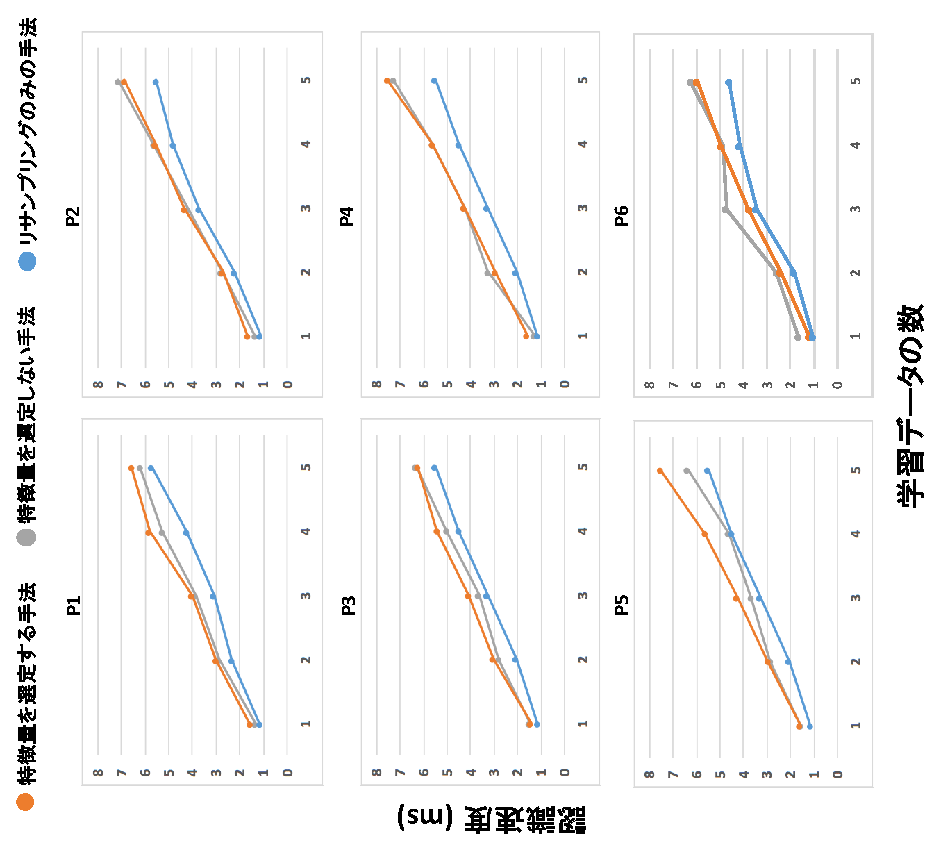
\includegraphics[width=0.9\columnwidth]{img/pre_speed.eps}
\caption{各手法における,被験者ごとの認識速度の平均}
\label{fig:rare_speed}
\end{figure}

\subsubsection{N-best Listの1番目と2番目のスコアの差}
図\ref{fig:rare_diff}に各手法ごとのN-best Listの1番目と2番目のスコアの差を示す.
N-best Listの1番目と2番目のスコアの差は,リサンプリングのみの手法,特徴量を選定する手法,特徴量を選定しない手法の順に大きくなった.
リサンプリングのみの場合においては,正規化しないため,類似するジェスチャとそれ以外のジェスチャにおいて,類似度の差が大きくなりやすくなったと言える.特徴量を選定する手法及び特徴量を選定しない手法は,正規化するため,類似度の差が大きくなりづらいが,特徴量を選定する手法は,ジェスチャグループの学習データ間の類似度が小さい特徴量のみ認識に用いているため,類似度の差が比較的大きくなったと言える.それに対し,特徴量を選定しない手法は識別に必要のない特徴量も認識に用いるため,例えば,向きが異なるが位置がほぼ同じであるジェスチャを識別しようとする場合に,位置の類似度を加味してしまい,類似度の差が小さくなったと言える.

\begin{figure}[!h]
\centering
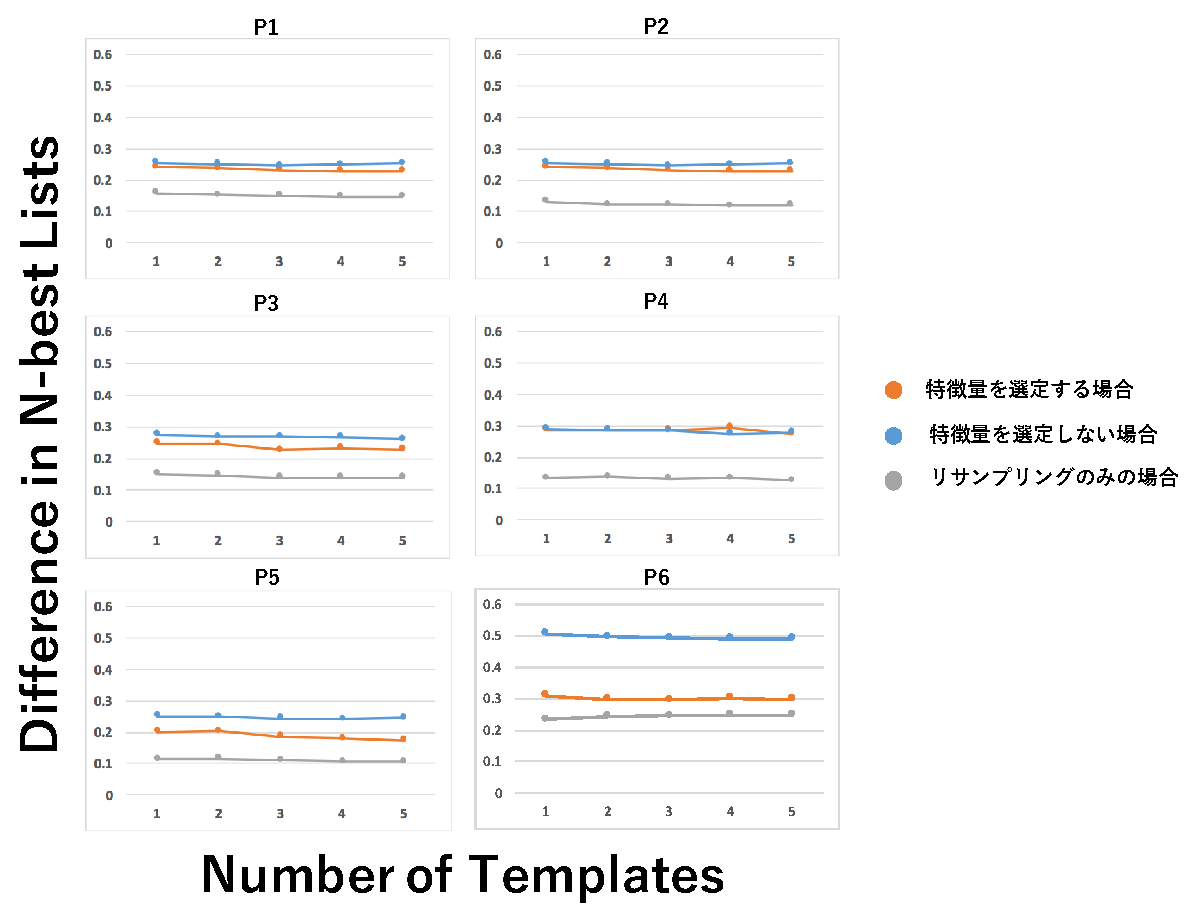
\includegraphics[width=0.9\columnwidth]{img/pre_diff.eps}
\caption{各手法における,被験者ごとのN-best Listの1番目と2番目のスコア差の平均}
\label{fig:rare_diff}
\end{figure}

\subsubsection{ジェスチャが正しく認識された時の類似度}
図\ref{fig:rare_sim}に各手法ごとのジェスチャが正しく認識された時の類似度を示す.
特徴量を選定する手法及び特徴量を選定しない手法は,ジェスチャが一致した時の類似度の平均値は高くなり,ほぼ同じような結果となった.特徴量を選定しない手法は,特徴量を選定する場合と比べて類似度が小さくなると予想されたが,類似度は高くなった.これは,本実験がユーザ依存であったため,被験者の書くジェスチャの再現率が高かったことが原因であると言える.リサンプリングのみの手法は被験者の書くジェスチャの再現率が高くとも,正規化しないため類似度が低くなったと言える.

\begin{figure}[!h]
\centering
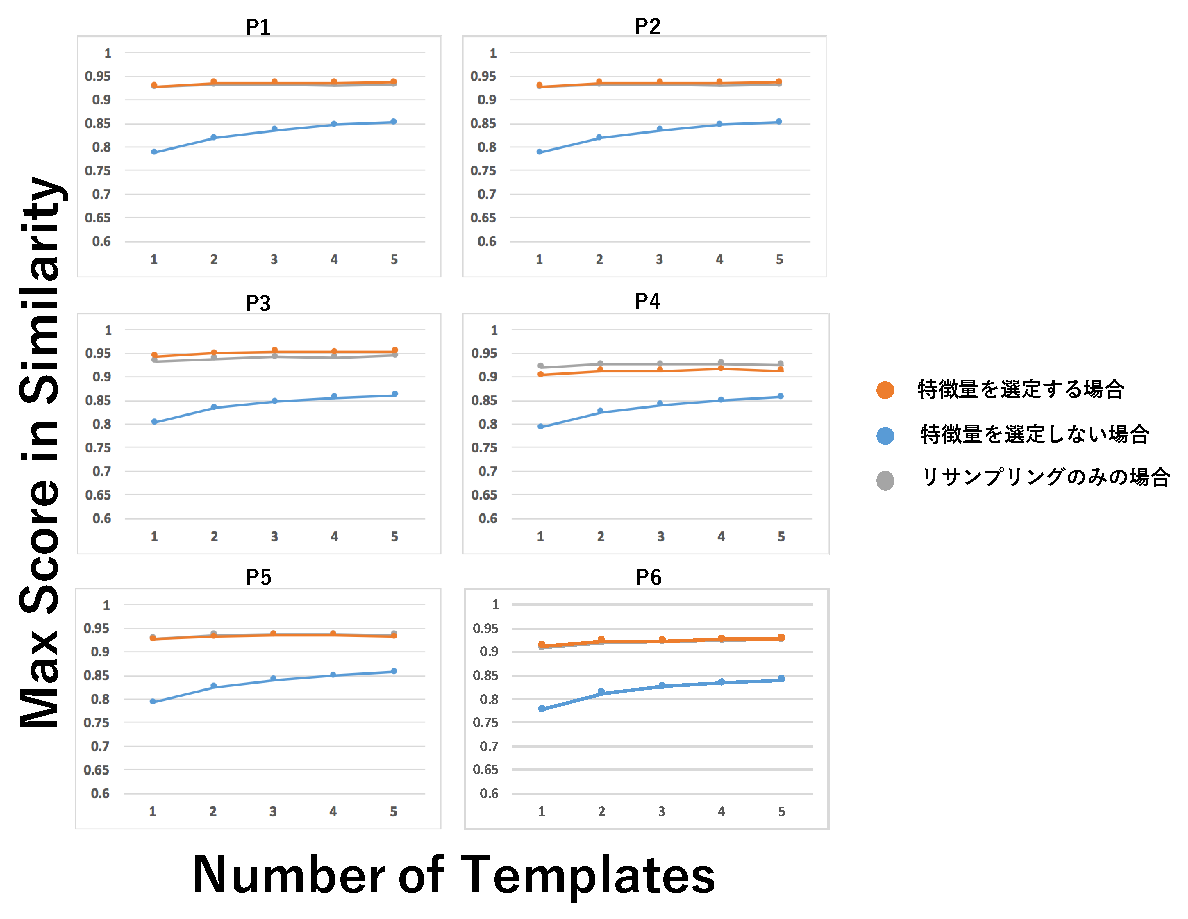
\includegraphics[width=0.9\columnwidth]{img/pre_sim.eps}
\caption{各手法における,被験者ごとのジェスチャが正しく認識された時の類似度の平均}
\label{fig:rare_sim}
\end{figure}

\newpage
\subsubsection{ジェスチャが正しく認識された時の類似度の最小値}
図\ref{fig:rare_min}に各手法ごとのジェスチャが正しく認識された時の類似度の最小値を示す.
特徴量を選定する手法及び特徴量を選定しない手法は,ジェスチャが一致した時の類似度の最小値は高くなった.また,リサンプリングのみの手法は低くなった.これらの要因は,ジェスチャが一致した時の類似度と同様であると考えられる.

\begin{figure}[!h]
\centering
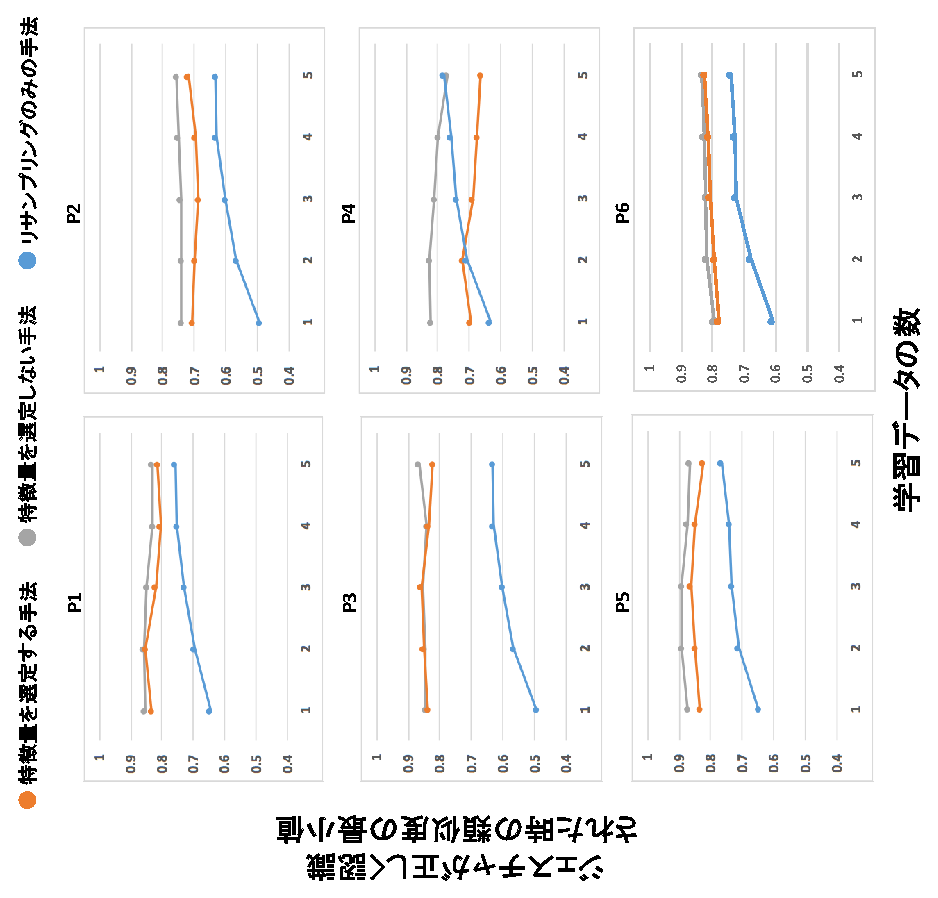
\includegraphics[width=0.9\columnwidth]{img/pre_min.eps}
\caption{各手法における,被験者ごとのジェスチャが正しく認識された時の類似度の最小値の平均}
\label{fig:rare_min}
\end{figure}

\newpage
\subsection{議論}

特徴量を選定する手法及び特徴量を選定しない手法はいずれも,認識率,認識速度のスコアは高く,特徴量を選定する手法はN-best Listの1番目と2番目のスコアの差も大きくなった.以上を踏まえ,
ジェスチャグループを作成し,ジェスチャグループ内に存在する学習データのみに対し,大きさ,向き,位置の類似度計算をすると認識速度の低下を抑えることができるという仮説及び,
同一ジェスチャグループ内において,他の学習データと類似している特徴量は,認識のための特徴量として用いなければ,認識率の低下を抑えることができるという仮説はある程度正しいと言える.それらに加え,特徴量を選定することによって,識別性能が向上するということも言える.

しかしながら被験者によっては,認識率及びN-best Listの1番目と2番目のスコアの差は小さくなった.この原因について考察する.

特徴量を選定する手法において,それぞれの特徴量は,認識に用いられるか用いられないかの二通りに分類され,閾値を設けることにより判別してきたが,ランダムに選ばれる学習データによっては,同じジェスチャグループであったとしても,認識に用いられる特徴量が異なる場合があった (閾値によって二通りのいずれかに分類されてしまうため,閾値の設定も難しいといった問題もある).

また,例えば図\ref{fig:group_similarity}に示すジェスチャグループにおいて,向き,位置が認識に用いる特徴量として選ばる可能性が高いが,向きは位置に比べ,類似度が小さい組み合わせが存在するため,向きの方が位置よりも識別するための特徴量としてより考慮されるべきではないのかという疑問や,それぞれの特徴量による類似度を,同じ尺度において扱うことができるのかという疑問があった (例えば,大きさの類似度 0.9 と向きの類似度 0.9 は,同じくらい類似していると言えるのかなど).

そこで,これらの問題点に対し,それぞれの特徴量を,認識に用いられるか用いられないかの二通りに分類するのではなく,特徴量に重み付けをすることによって解決しようと試みた.例えば,図\ref{fig:group_similarity}の場合,それぞれの特徴量に対する重みの和が1となる場合,これまでは特徴量を用いるか用いないかであったため,~(大きさ,向き,位置)の重みが~(0,0.5,0.5)であったところを,~(0.1,0.6,0.3)といった具合にする.
このように重みを導入することによって,認識に用いる特徴量をより高い尤度によって決定することを試みた.

そこで,我々は,認識率及びN-best Listの1番目と2番目のスコアの差を向上させる重みを求めることにした.

%\begin{figure} [h!]
%	\begin{center}
%		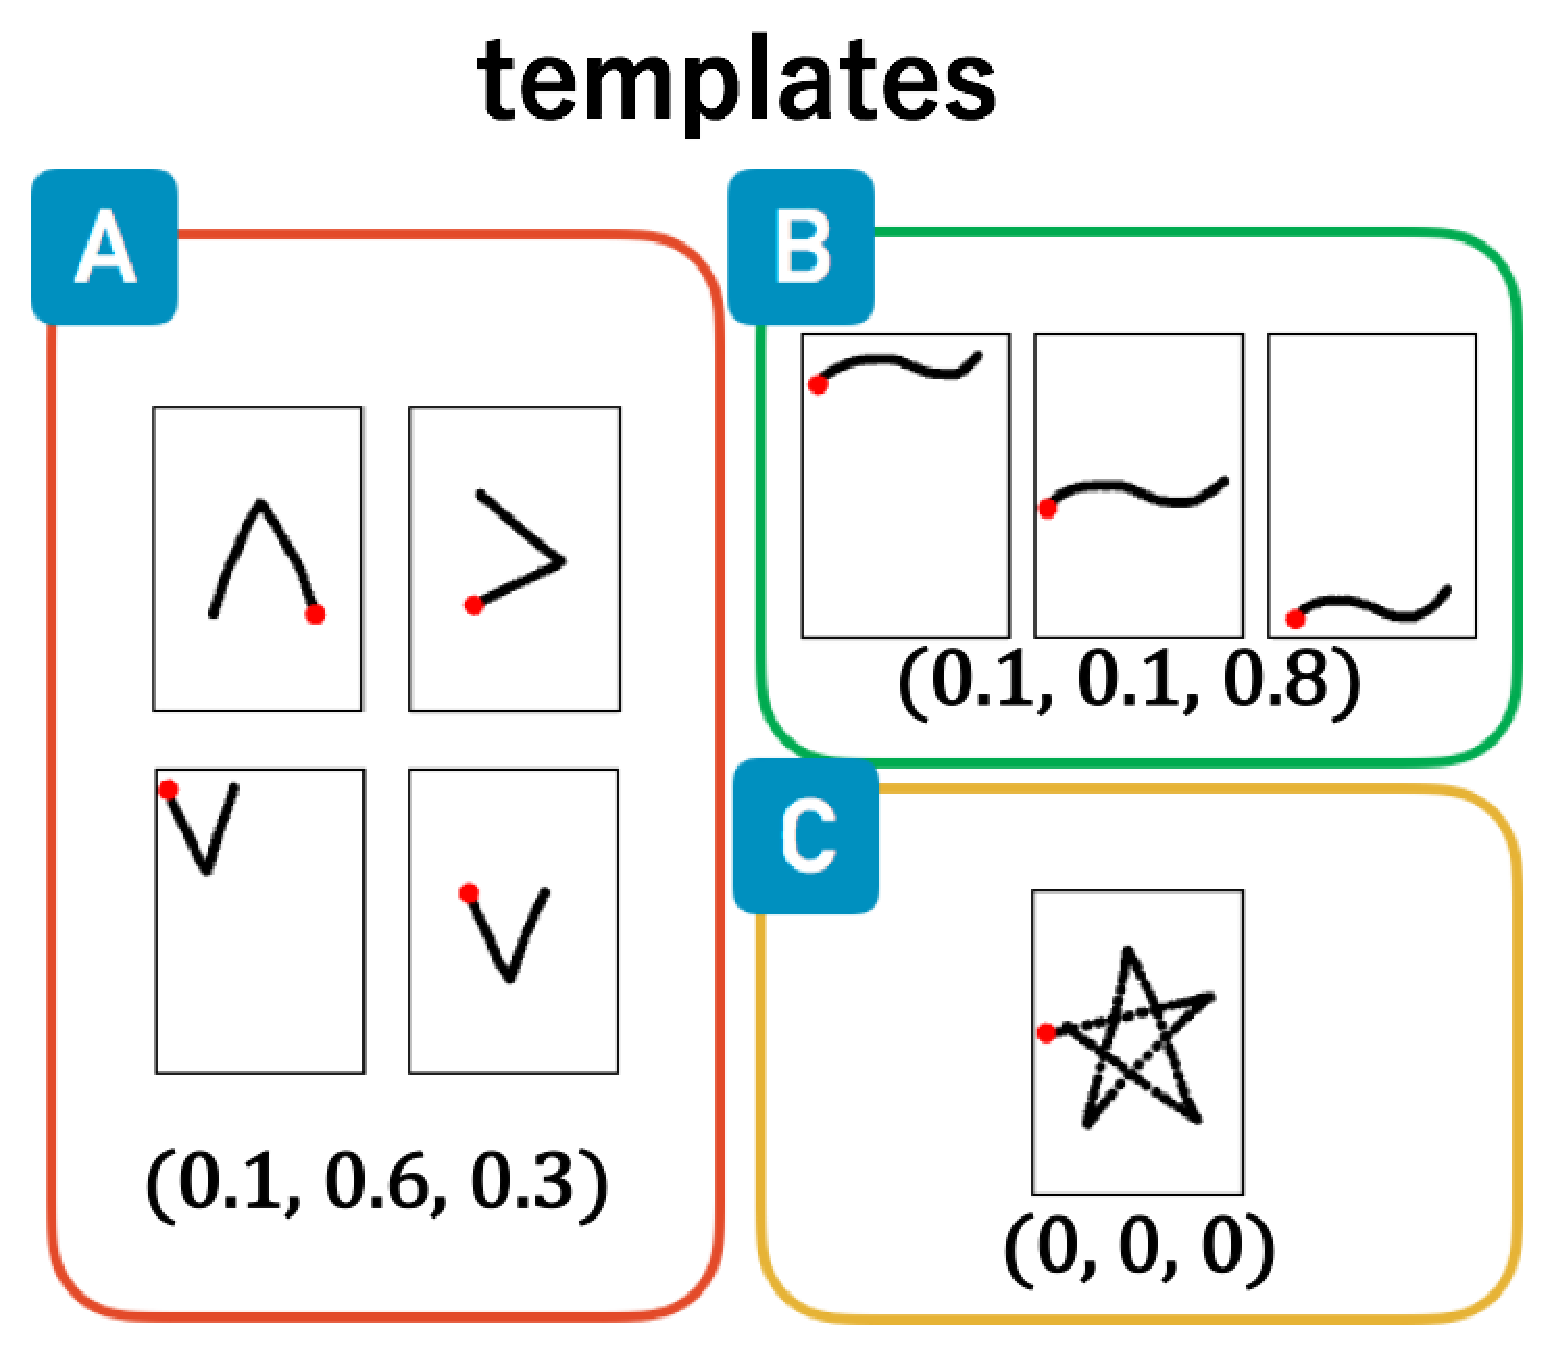
\includegraphics [width=0.7\hsize ]{img/group_weight.eps}
%	\end{center}
%	\caption{Examples of gesture groups and optimal weight values ($Ws$, $Wo$, $Wp$) for each group.}
%	\label{fig:group_weight}
%\end{figure}

\section{重み付けのための実験}
%「同一ジェスチャグループ内において,他の学習データと類似している特徴量は,認識のための特徴量として用いなければ,認識率の低下を防ぐことができる」という仮説
あるジェスチャグループが認識に用いるべき特徴量が,ジェスチャグループの学習データ間の類似度と関係していることは,これまで述べてきた通りである.
そこで我々は,ジェスチャグループの学習データ間の類似度をもとに,認識率及びN-best Listの1番目と2番目のスコアの差を向上させるための,それぞれの特徴量に対する重み付けの方法を実験的に求めることとした.

\subsection{重み付けの手順}
まず,重み付けの手順を述べる.

学習データは,追加されるたびに,\$1アルゴリズムを用いてジェスチャグループとして保管される.その際のジェスチャグループの決め方と,ジェスチャグループの学習データ間の類似度の計算方法は,5.3.2節及び5.3.3節に示したとおりである.

全ての学習データを追加し終わった後,入力データを入れていく.
まず\$1アルゴリズムによりどの形状のジェスチャであるかを判定する.これは5.3.4節において述べた方法と同じである.
その後,ジェスチャグループにおける大きさ,向き,位置のそれぞれの特徴量に対する重みを求める手順へと移行する.その方法を図\ref{fig:weight_method1},図\ref{fig:weight_method2}に図示する.
まず,入力データと学習データの類似度を求める.その後大きさ,向き,位置のそれぞれの特徴量に対する重みを,それぞれの和が1となるようにそれぞれ0.1ずつ変化させていく.そして,重みを先ほど求めた類似度に式5.8に則って乗算することによって,最終的な類似度を求める.ここで,式5.8において, $S_\textit{cs}$は入力データと学習データの大きさの類似度,$S_\textit{co}$は入力データと学習データの向きの類似度,$S_\textit{cp}$は入力データと学習データの位置の類似度を示しており,$W_\textit{s}$は大きさの重み,$W_\textit{o}$は向きの重み,$W_\textit{p}$は位置の重みを示している.これを各ジェスチャセットに含まれる,全てのジェスチャについて行う.この時,ジェスチャが一致した時の類似度の平均値が0.9以上,N-best Listの1番目と2番目のスコアの差が0.2以上の時のそれぞれの特徴量に対する重みを記録する.これを各被験者から得られた各ジェスチャセットごとに行う.

このようにして,各ジェスチャセットから得られる,それぞれのジェスチャグループ内の学習データ間の類似度と,重みをセットにして記録することによって,どのような特徴を持つジェスチャグループの場合に,どのような重み付けをすることが望ましいかを考察する.

\begin{equation}
S_\textit{final} = S_\textit{cs} \times W_\textit{s} + S_\textit{co} \times W_\textit{o} + S_\textit{cp} \times W_\textit{p}
\end{equation}

\begin{figure} [h!]
	\begin{center}
		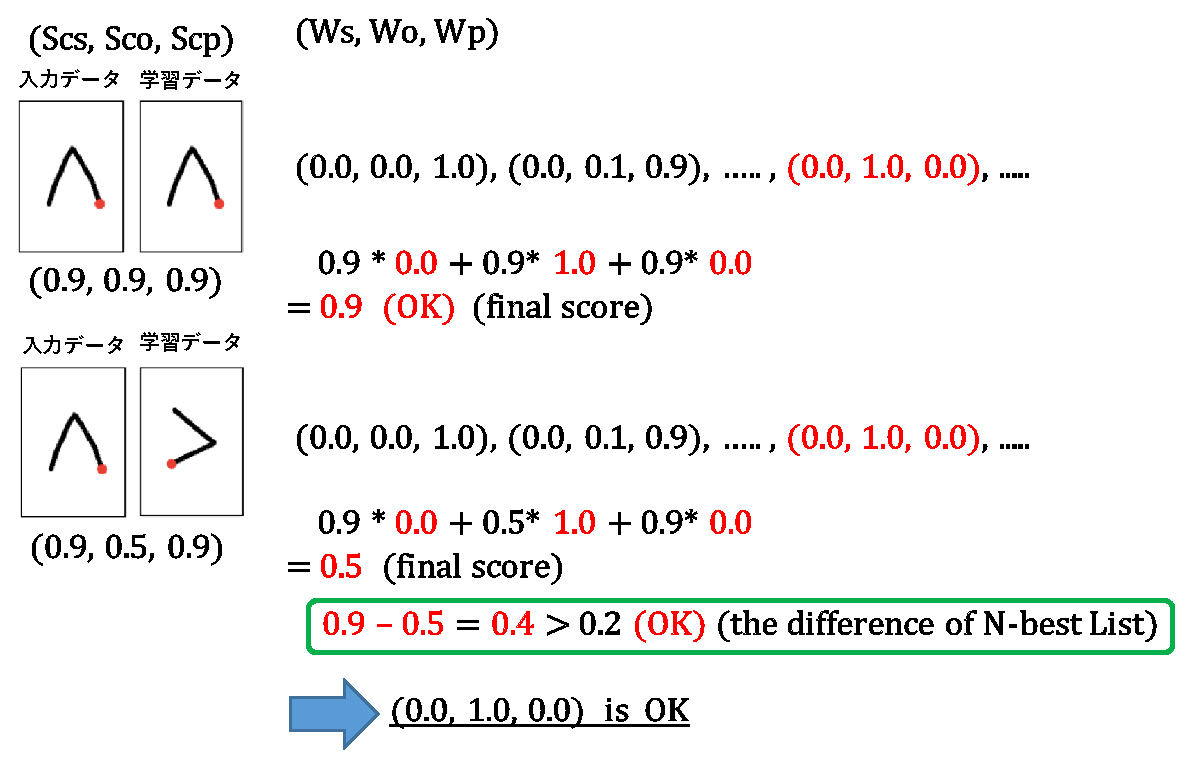
\includegraphics [width=0.8\hsize ]{img/weight_method2.eps}
	\end{center}
	\caption{条件を満たす重みが決定されるまでの手順}
	\label{fig:weight_method1}
\end{figure}

\begin{figure} [h!]
	\begin{center}
		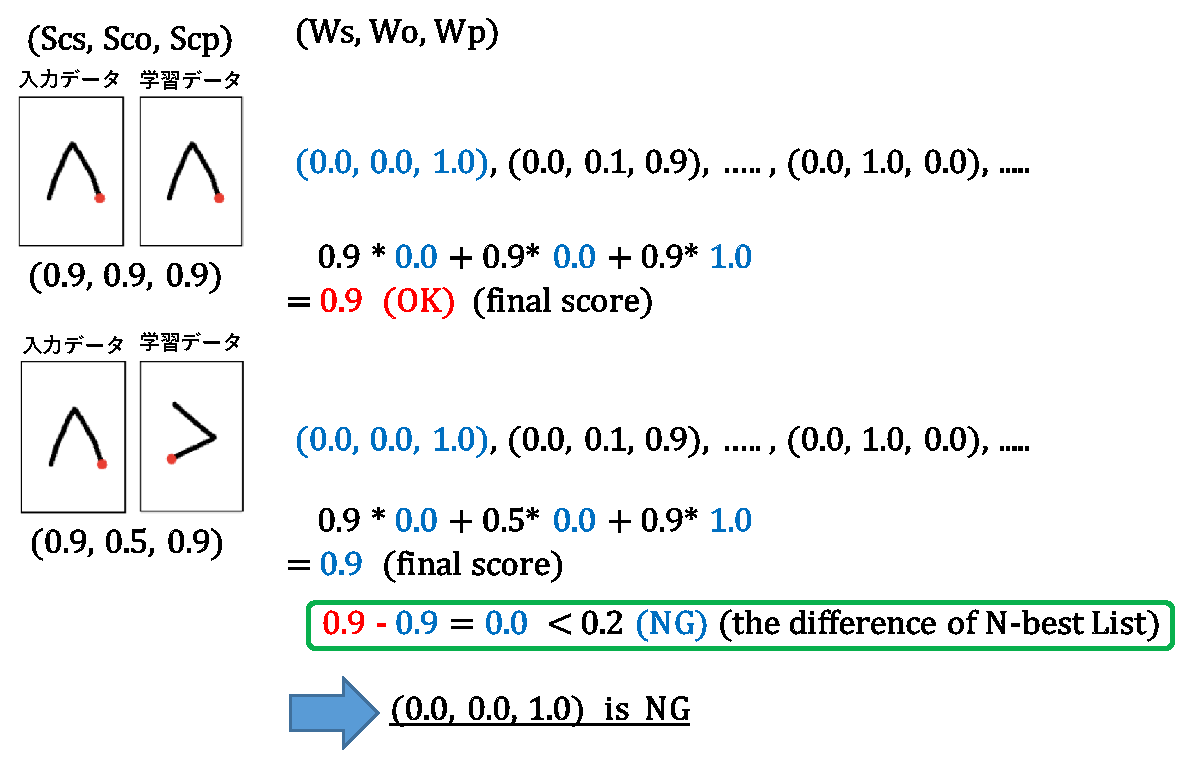
\includegraphics [width=0.8\hsize ]{img/weight_method1.eps}
	\end{center}
	\caption{条件を満たさない重みが決定されるまでの手順}
	\label{fig:weight_method2}
\end{figure}

\clearpage
\subsection{実験結果}
%最適な重み付けのための実験結果を示す.

図\ref{fig:weight_size}は,ジェスチャグループ内の学習データ間の類似度と大きさの重みの関係,
図\ref{fig:weight_orientation},ジェスチャグループ内の学習データ間の類似度と向きの重みの関係,
図\ref{fig:weight_position}は,ジェスチャグループ内の学習データ間の類似度と位置の重みの関係の結果を被験者ごとに示している.
ここで,$S_\textit{ts}$はジェスチャグループの学習データ間の大きさの類似度,$S_\textit{to}$はジェスチャグループの学習データ間の向きの類似度,$S_\textit{tp}$はジェスチャグループの学習データ間の位置の類似度を示している.

ある類似度の時の条件を満たす重みは複数存在するため,プロットされているデータは,その平均値と標準偏差である.

\begin{figure}[!h]
\centering
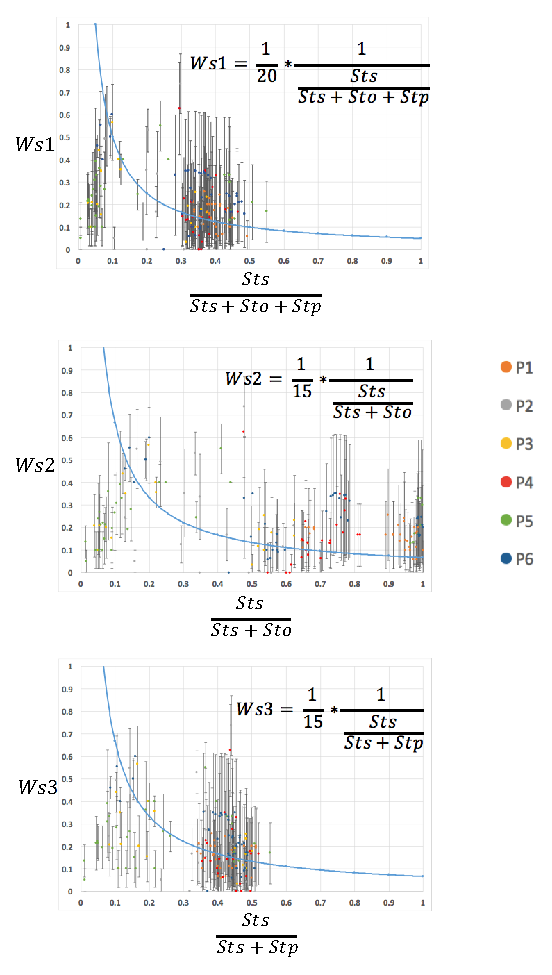
\includegraphics[width=0.7\columnwidth]{img/weight_size.eps}
\caption{ジェスチャグループ内の学習データ間の類似度と大きさの重みの関係の被験者ごとの結果}
\label{fig:weight_size}
\end{figure}

\begin{figure}[!h]
\centering
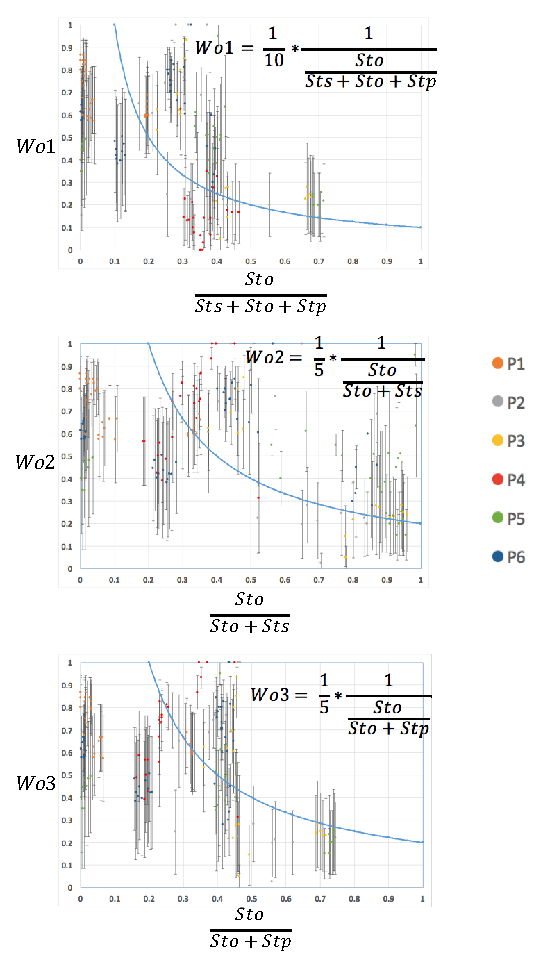
\includegraphics[width=0.7\columnwidth]{img/weight_orientation.eps}
\caption{ジェスチャグループ内の学習データ間の類似度と向きの重みの関係の被験者ごとの結果}
\label{fig:weight_orientation}
\end{figure}

\begin{figure}[!h]
\centering
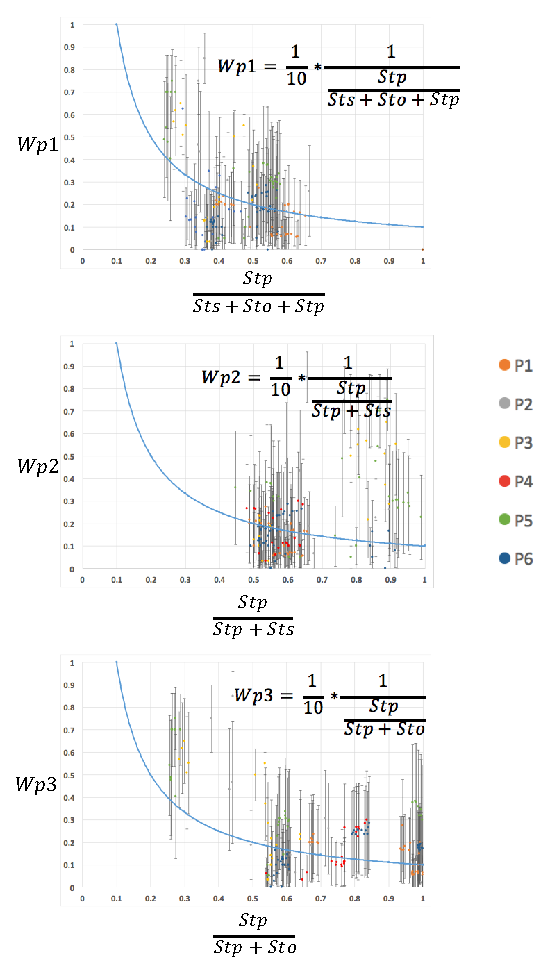
\includegraphics[width=0.7\columnwidth]{img/weight_position.eps}
\caption{ジェスチャグループ内の学習データ間の類似度と位置の重みの関係の被験者ごとの結果}
\label{fig:weight_position}
\end{figure}

それぞれについて,我々はジェスチャグループ内の学習データ間の類似度と重みを関係式によって表すこととした.
関係式は,それぞれのグラフにおいて青色の線によって示されており,グラフの右上に式が示されている.

この関係式の求め方について述べる.

まず,実験から得られたジェスチャグループ内の学習データ間の類似度と重みの関係の近似式を求める.
この時,両対数グラフにおいて,およそ直線で表せられることがわかった.つまり,これらの関係は累乗近似曲線に近似できることがわかった.
しかしながら,近似された累乗近似曲線に対し値が離れている元データが多く存在するため,近似式がどれほど元データを表すものになっているかを示す決定係数$R^2$は,どのグラフにおいても低くなった.

そこで我々は,累乗近似曲線に近似できることを手掛かりに,近似式を以下のように定めた.\begin{equation}
W = \frac{1}{α} \times \frac{1}{S} 
\end{equation}
ここで,Wは重み,Sは類似度を示す.

そして,αを5〜30まで5ずつ増やし,その時に求められる重みを元に認識率を測定したところ,図\ref{fig:weight_size}〜図\ref{fig:weight_position}において示されるような近似式において,認識率が高くなることがわかった.

\clearpage
\section{重みを用いたジェスチャの認識}
以上を踏まえ,重みを用いたジェスチャ認識が可能となる.

まず,学習データを追加する際に,ジェスチャグループ内の学習データ間の類似度を元に重みを求める.
この際,図\ref{fig:weight_size}〜図\ref{fig:weight_position}において示される近似式を元に重みを求める.これは,以下の式に統合される.
\begin{equation}
W_\textit{s} = \frac{1}{90}(5.5 + 3.5\frac{S_\textit{to} + S_\textit{tp}}{S_\textit{ts}})
\end{equation}
\begin{equation}
W_\textit{o} = \frac{1}{30}(5.0 + 3.0\frac{S_\textit{ts} + S_\textit{tp}}{S_\textit{to}})
\end{equation}
\begin{equation}
W_\textit{p} = \frac{1}{30}(3.0 + 2.0\frac{S_\textit{ts} + S_\textit{to}}{S_\textit{tp}})
\end{equation}
ここで,$S_\textit{ts}$は学習データ間の大きさの類似度,$S_\textit{to}$は学習データ間の向きの類似度,$S_\textit{tp}$は学習データ間の位置の類似度を示している.


次に,実際に入力データを認識させる手順を述べる.
\begin{enumerate}
\item \$1アルゴリズムを用いることにより,どのジェスチャグループに属するか判別する.この時,学習データを追加する時と同様,ジェスチャグループ内のすべての学習データに対し類似度を求め,0.8を超えた場合あるいは,0.8を超えるジェスチャが複数存在する場合は,最も類似度が高いジェスチャが存在するジェスチャグループに属すると判別する.
\item 1.によって判別されたジェスチャグループ内において,どのジェスチャと最も類似しているかを判別する.

この際,ジェスチャグループ内において,入力データと学習データの類似度~($S_\textit{cs}$,$S_\textit{co}$,$S_\textit{cp}$)を求め,学習データを追加した際に式5.10〜式5.12によって求めた重みを用い,式5.8によって最終的な類似度を求める.この類似度が最も高かった時のジェスチャが判別されるジェスチャとなる.

\end{enumerate}

この重み付けを考慮したアルゴリズムを,\$Vの最終的なアルゴリズムとする.








%評価実験
\chapter{評価実験}
本章にて,重み付けを考慮した\$Vアルゴリズムの性能評価実験を述べる.

\section{実験設計}
\$Vの認識率,認識速度,類似度のN-best Listの1番目と2番目のスコアの差,ジェスチャが一致した時の類似度,ジェスチャが一致した時の類似度の最小値を測定することによってアルゴリズムの性能を評価した.また,認識率,認識速度に関しては,\$Vの拡張元である\$1及び,\$Vと同様に,大きさ,向き,位置に関して異なる手書きジェスチャを識別可能なRubine,DTWと比較した.

実験に用いたジェスチャは,5章と同様,ユーザ調査によって得られたジェスチャを用いる.
また,それぞれの測定方法については,5章において述べた通りに行うが,\$1については,大きさ,向き,位置に関して手書きジェスチャを識別できないため,形状と書き順さえ正しく認識されれば,正しく認識されたとみなした.

\section{実験結果と考察}
\subsection{認識率}
\begin{figure}[!h]
\centering
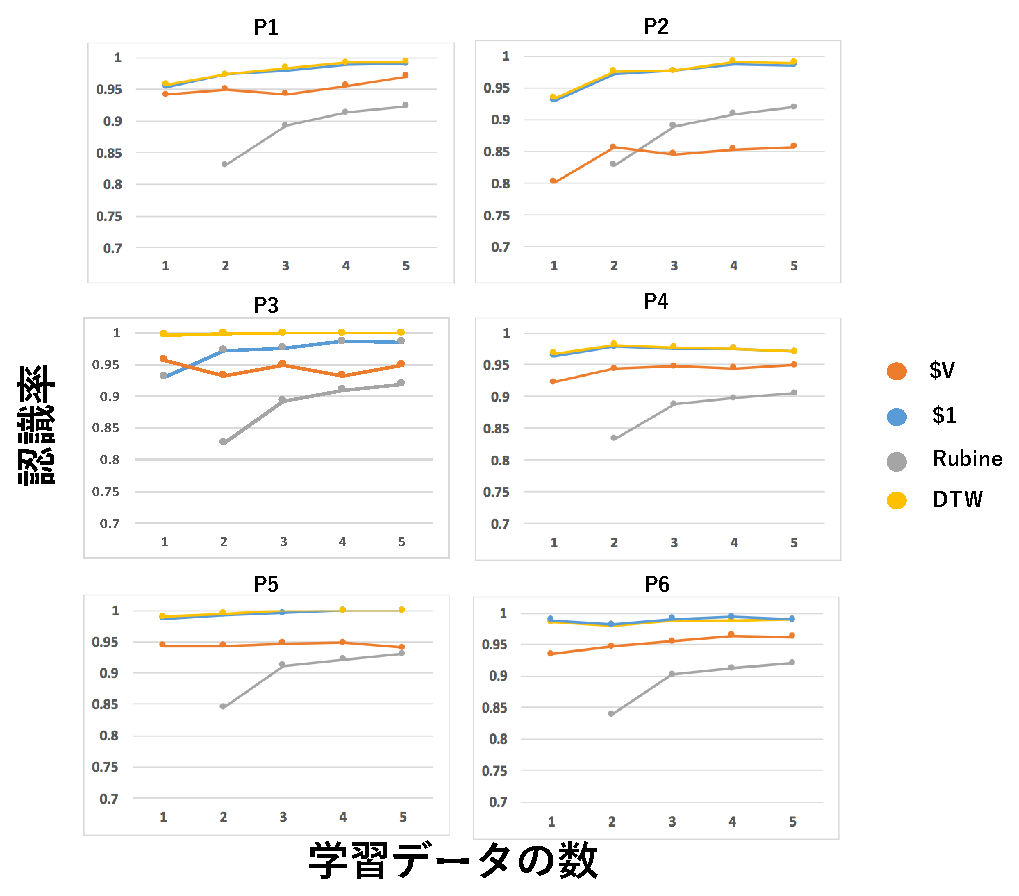
\includegraphics[width=1.0\columnwidth]{img/rec_rate.eps}
\caption{各手法における,被験者ごとの認識率の平均}
\label{fig:rec_rate}
\end{figure}

図\ref{fig:rec_rate}に各手法ごとの認識率の結果を示す.
それぞれの被験者の平均は,\$Vは93\%~(SD=4.55),\$1は98\%~(1.04),DTWは98\%~(0.86),Rubineは88\%~(2.14)であった.\$Vは\$1とDTWに対し,有意に低かった(p $<$ 0.01)が,被験者P1,P3,P4,P5,P6に関しては認識率の平均は95\%~(1.27)と高く,\$1と比べて認識率の低下を最小限に抑えることができた.\$Vは\$1とは異なり,大きさ,向き,位置に関して異なる手書きジェスチャを識別可能であるにもかかわらず,被験者P1,P3,P4,P5,P6に関しては,認識率はおよそ3\%しか低下しなかった.Rubineと比較した場合は,P1,P3,P4,P5,P6に関しては\$Vは有意に高かった(p $<$ 0.001).また,重み付けをしない場合と比べても,\$Vは全被験者について認識率は向上した.

P2の認識率が低かったのは,P2は別の名前のジェスチャで,形状が酷似したジェスチャが複数存在したため,識別が困難になったことが要因であると考えられる.また,\$Vは学習データに比例して認識率が高くなるとは言えない.これは,同じジェスチャの学習データを追加するたびに,大きさ,向き,位置それぞれの特徴量を算術平均するため,必ずしも入力データに類似する学習データが存在する可能性が高くなるとは言えないからである.しかしながら,ほとんどの被験者において,少ない学習データにおいて高い認識率を示し,学習データが1つの場合における,全ジェスチャセットの認識率の平均は91.2\%(SD=0.07),学習データが2つの場合は92.2\%(0.04),学習データが3つの場合は92.7\%(0.05),学習データが4つの場合は93.3\%(0.04),学習データが5つの場合は93.2\%(0.05)となった.

\newpage
\subsection{認識速度}
\begin{figure}[!h]
\centering
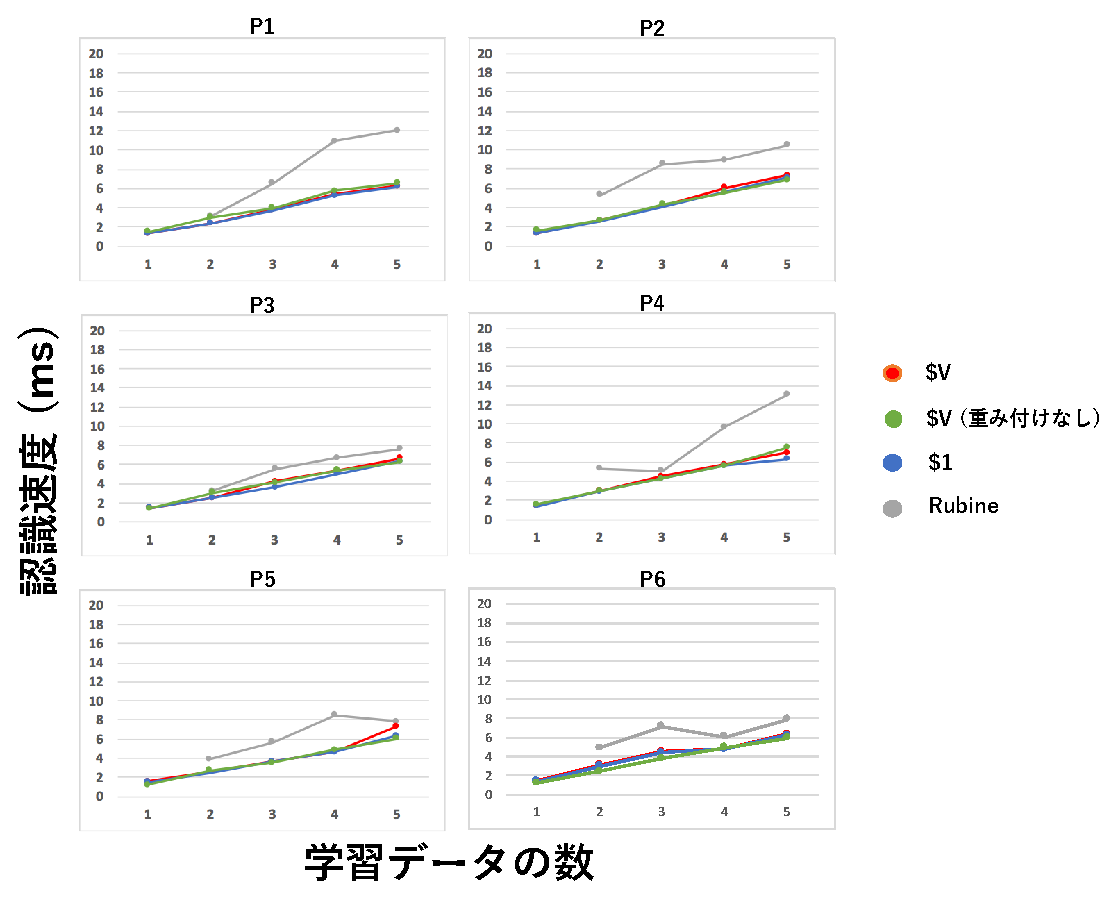
\includegraphics[width=1.0\columnwidth]{img/rec_speed.eps}
\caption{\$V,\$1,Rubineにおける,被験者ごとの認識速度の平均}
\label{fig:rec_speed}
\end{figure}

\begin{figure}[!h]
\centering
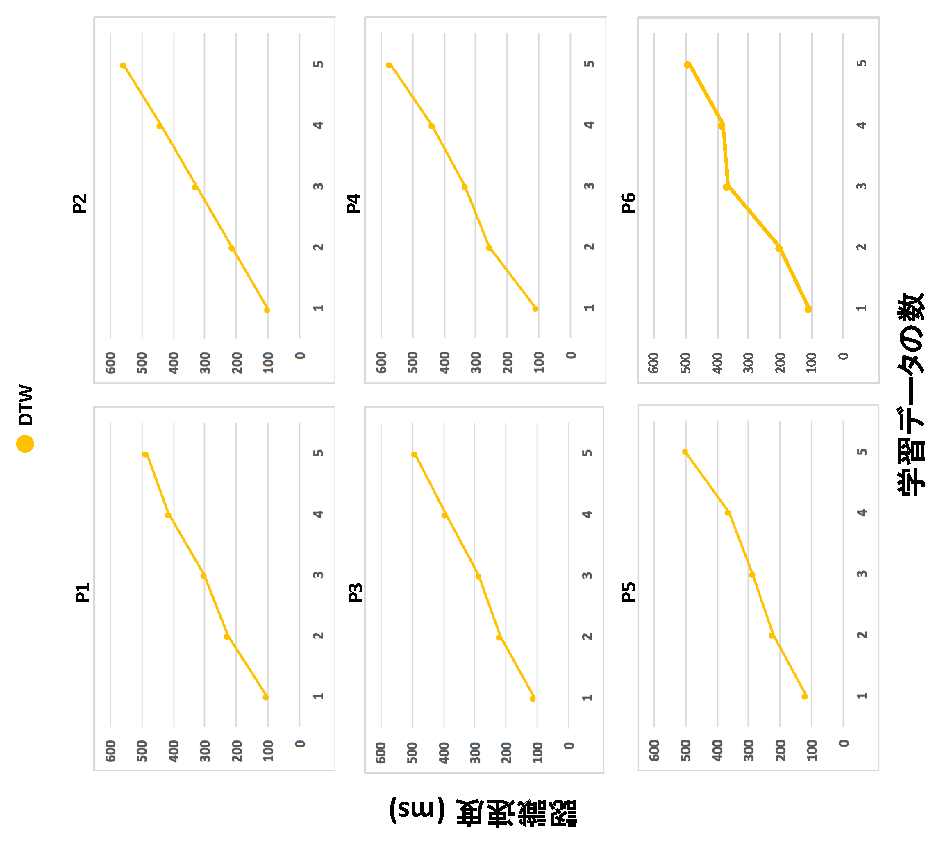
\includegraphics[width=1.0\columnwidth]{img/rec_speed_dtw.eps}
\caption{DTWにおける,被験者ごとの認識速度の平均}
\label{fig:rec_speed_dtw}
\end{figure}

図\ref{fig:rec_speed}に,\$V,\$1,Rubineの,図\ref{fig:rec_speed_dtw}に,DTWのジェスチャ1つを認識するまでの認識速度の結果を示す.
\$Vの認識速度は,全被験者の平均が,学習データの数が1つの場合~2.6ms (SD=0.2),学習データの数が2つの場合~3.5ms (0.3),学習データの数が3つの場合~4.1ms (0.3),学習データの数が4つの場合~4.9ms (0.3),学習データの数が5つの場合~6.1ms (0.4)となり非常に速いと言える.また,\$1と認識速度に有意差はなく~(p $<$ 0.001),\$Vは\$1と比べて認識速度の低下を抑えることに成功した.Rubineと比べると有意に速かった~(p $<$ 0.005).DTWの認識速度は図\ref{fig:rec_speed_dtw}に示すように非常に遅く,\$Vの認識速度はDTWのおよそ100分の1であった.
また,学習データに比例して認識速度が遅くなることも分かった.

\clearpage
\subsection{識別性能の結果}
\$Vの識別性能の結果を,N-best Listの1番目と2番目のスコアの差及びジェスチャが正しく認識された時の類似度及びジェスチャが正しく認識された時の類似度の最小値を示すことによって述べる.

図\ref{fig:rec_diff}に\$VにおけるN-best Listの1番目と2番目のスコアの差,図\ref{fig:rec_sim}に\$Vにおけるジェスチャが正しく認識された時の類似度,図\ref{fig:rec_min}に\$Vにおけるジェスチャが正しく認識された時の類似度の最小値の結果を示す.
N-best Listの1番目と2番目のスコアの差について,全ジェスチャセットの平均値はおよそ0.24~(SD = 0.10)となった.また,ジェスチャが正しく認識された時の類似度の平均値は0.94~(SD=0.04)となり非常に高いと言えるが,ジェスチャが正しく認識された時の類似度の最小値は被験者によってばらつきが生じ,平均値はおよそ0.83~(0.14)であった.また,N-best Listの1番目と2番目のスコアの差は,重み付けをしない場合と比べて有意に高く~(p $<$ 0.01),識別性能が向上したと言える.しかしながら,ジェスチャが正しく認識された時の類似度の最小値は,重み付けをしない場合と比べて有意に低かった~(p $<$ 0.01).これは,ジェスチャグループによっては,適した重み付けがされていない場合があり,その場合類似度が低くなるからであると考えられる.以上を踏まえ,%ジェスチャが正しく認識された時の類似度の平均値が高いことから,
重み付けは多くのジェスチャグループにおいて適用可能であるが,適用することによって類似度が低下する場合もあることがわかった.
また,ジェスチャが一致した時の類似度の最小値の平均は0.65以上であり,N-best Listの1番目と2番目のスコアの差の平均値は0.15以上であることから,認識のための類似度の閾値を0.5とすることによって,ジェスチャが一致するか否かを判別することが可能となると言える.
%\subsubsection{N-best Listsの1番目と2番目のスコアの差}
\begin{figure}[!h]
\centering
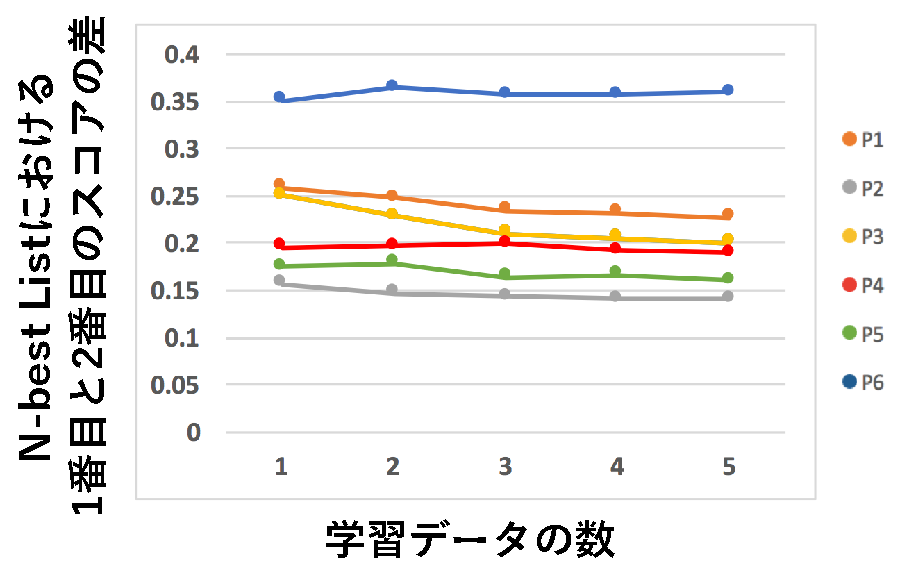
\includegraphics[width=0.7\columnwidth]{img/rec_diff.eps}
\caption{\$Vにおける,N-best Listの1番目と2番目のスコアの差の平均}
\label{fig:rec_diff}
\end{figure}

%\subsubsection{ジェスチャが正しく認識された時の類似度}
\begin{figure}[!h]
\centering
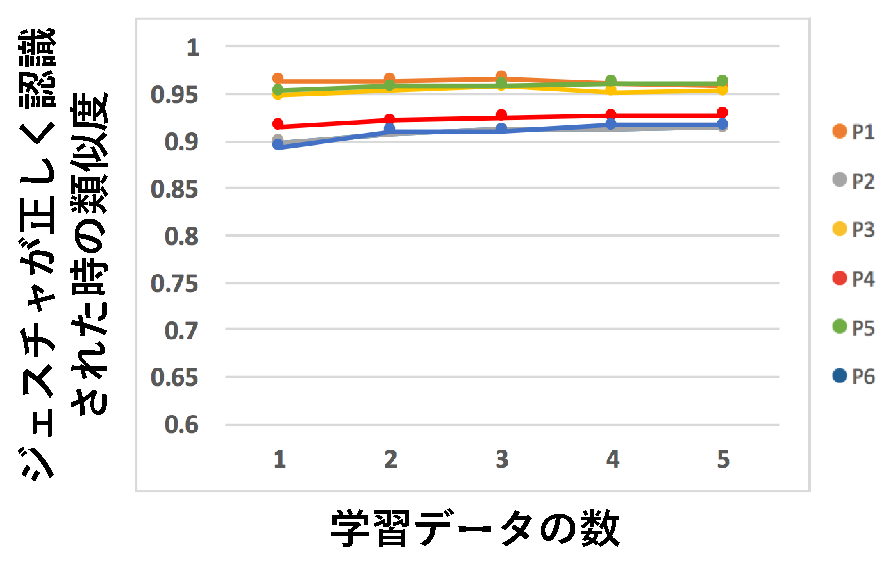
\includegraphics[width=0.7\columnwidth]{img/rec_sim.eps}
\caption{\$Vにおける,ジェスチャが正しく認識された時の類似度の平均}
\label{fig:rec_sim}
\end{figure}

%subsubsection{ジェスチャが正しく認識された時の類似度の最小値}
\begin{figure}[!h]
\centering
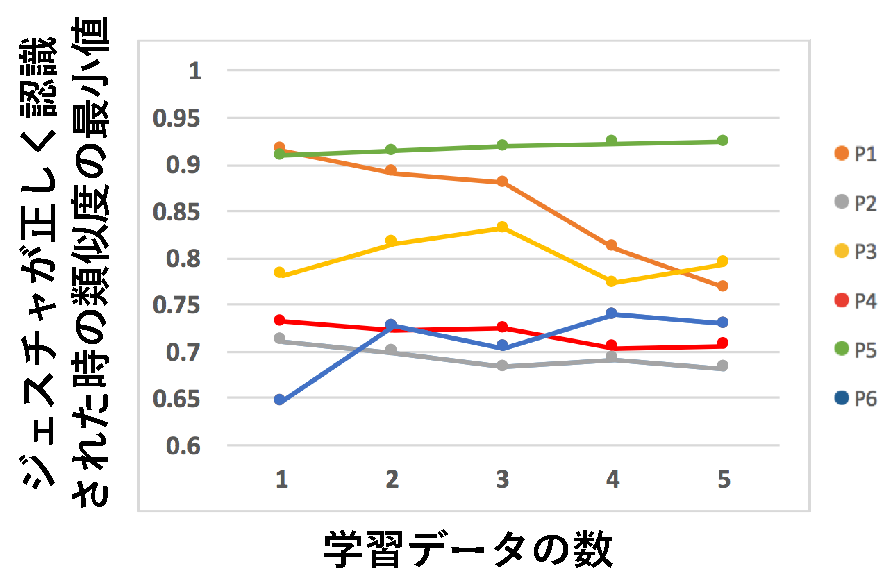
\includegraphics[width=0.7\columnwidth]{img/rec_min.eps}
\caption{\$Vにおける,ジェスチャが正しく認識された時の類似度の最小値の平均}
\label{fig:rec_min}
\end{figure}

\clearpage
以上を踏まえ,ジェスチャグループを作成し,ジェスチャグループ内に存在する学習データのみに対し,大きさ,向き,位置の類似度計算をすると認識速度の低下を防ぐことができるという仮説及び,同一ジェスチャグループ内において,他の学習データと類似している特徴量は,認識のための特徴量として用いなければ,認識率の低下を防ぐことができるという仮説は検証され,\$Vは,認識率及び認識速度において高いパフォーマンスを示し,かつ,形状や書き順が同じ手書きジェスチャを大きさ,向き,位置に関して識別可能なアルゴリズムであると言える.

%\TODO{学習データを追加する際の計算量を計測}


%アプリケーション例
\chapter{アプリケーション例}
\$Vを利用したアプリケーション例を本章において示す.
\$Vは少ない学習データにおいて,高い認識率及び識別性能を示すため,ユーザ定義ジェスチャを利用したアプリケーションを開発することができる.
また,同じ形状及び書き順の手書きジェスチャを大きさ,向き,位置に関して識別可能であるため,それらを利用したアプリケーション例を示す.

\section{手書きジェスチャを利用したアプリケーション開発ツールキット}
まず,ユーザは,入力として用いたい手書きジェスチャを学習データとして追加していく~(図).
すると,\$Vが実装された本ツールキットは,追加された学習データを自動的にジェスチャグループに分類し,それぞれのジェスチャグループごとに,大きさ,向き,位置の特徴量に対する最適な重みを自動計算する~(図).
最後に,ユーザは,あるアプリケーションにおける処理を実行するAppleScriptあるいはボタンと手書きジェスチャを対応付けることによって~(図),手書きジェスチャを利用したアプリケーションを開発することができる.


このツールキット使うことによって,例えば,図のようなメディアプレイヤを開発することができる.
このメディアプレイヤにおいて,再生,巻き戻し,前のメディア,次のメディアなどに対し,同じ書き順及び同じ形状の手書きジェスチャが割り当てられており,それぞれ,大きさ,向きの違いが利用されている.
このようにして,大きさ,向き,位置の違いを利用することによって,より実際の動作に即した手書きジェスチャを割り当てることが可能となる.
また,大きさ,向き,位置の違いを利用できない場合と比べて,利用可能な手書きジェスチャの種類が大きく拡大し,アプリケーションユーザが入力として用いたい手書きジェスチャを考案しやすくなったと言える.


%議論
\chapter{議論}
7章までにおいて,\$Vアルゴリズムの詳細及び性能評価を述べた.
本章において,\$Vが今後どのように改善されうるか,あるいは\$Vをどのように発展利用できるかについて議論する.

\section{最適な重み付けの再定義}
5.4節において,認識率及びN-best Listの1番目と2番目のスコアの差を向上させるための重みを実験的に求めた.
しかしながら,ジェスチャグループ内の学習データ間の類似度と重みの関係を示す近似式の決定係数$R^2$は高いとは言えず,今回は,式5.9において示されるように変数を1つにし,段階的に変化させることによって近似式を求めた.
このように決定係数$R^2$が低くなった要因は,ジェスチャグループ内の学習データ間の類似度と重みは,ある程度相関を示したものの,データにばらつきが存在したことであると考えられる.

今回,このデータは,あるジェスチャグループ内の学習データ間の類似度において,ジェスチャが一致した時の類似度の平均値が0.9以上,N-best Listの1番目と2番目のスコアの差が0.2以上となる重みの平均値としてプロットされている.しかしながら,当然ながらこの条件を満たす多くの重みにおいて,具体的な類似度の平均値及びN-best Listの1番目と2番目のスコアの差には違いがある~(例えば,類似度が0.9,N-best Listの1番目と2番目のスコアの差が0.2である重みも存在すれば,類似度が0.99,N-best Listの1番目と2番目のスコアの差が0.4である重みも存在する).このことから,条件を満たす重みを平均するのではなく,高いスコアを示す重みをより重要視することによって,データのばらつきを抑えられる可能性がある.
データのばらつきを抑えることによって,近似式の決定係数$R^2$は高くなり,よりデータを忠実に表す近似式を得られ,認識率の向上あるいは識別能力の向上を実現できるかもしれない.


\section{ユーザに依存しない手書きジェスチャの精度評価}
本研究において,ジェスチャを定義したアプリケーションユーザが,自身が定義したジェスチャを入力した時に,\$Vがどれだけ認識できるかを評価した.今回はアプリケーションユーザが手書きジェスチャ定義する場合を想定しているため,ユーザに依存した手書きジェスチャの評価を行った.しかしながら,アプリケーション開発者が手書きジェスチャを定義する場合,実際に入力するのはアプリケーションユーザであるため,ユーザに依存しない手書きジェスチャにおいても,高い認識率及び高い識別性能が求められる.\$Vは識別に必要のない特徴量の重みを小さくするなどの処理を施すことによって,ロバスト性を極力維持しているため,ユーザに依存しない手書きジェスチャにおいて,
重み付けをしない場合と比べて,高い認識率及び高い識別能力を示す可能性が高い.また,\$1,DTW,Rubineとの比較を含め,ユーザに依存しない手書きジェスチャの精度評価を行うことによって,さらなる改善の余地を発見できるであろう.


\section{書き順に依存しないアルゴリズムの導入}
\$Vは\$1の拡張であり,\$1と同様に形状と書き順を同じジェスチャを認識することができるため,図\ref{fig:different_direction}のような形状が同じであっても書き順の異なるジェスチャは別のジェスチャとして認識される.双方を同じジェスチャとして認識してほしい場合には,それぞれのジェスチャを同じ名前で登録する必要がある.
このようなアプリケーションユーザへの負担を解消すべく,書き順に依存しない,つまり形状さえ同じであれば同じジェスチャとみなすアルゴリズムは\$N~\cite{Anthony:2010:LMR:1839214.1839258}において開発されているため,このアルゴリズムを活用することによって書き順に依存しないアルゴリズムを実現することができる.

\begin{figure} [h!]
	\begin{center}
		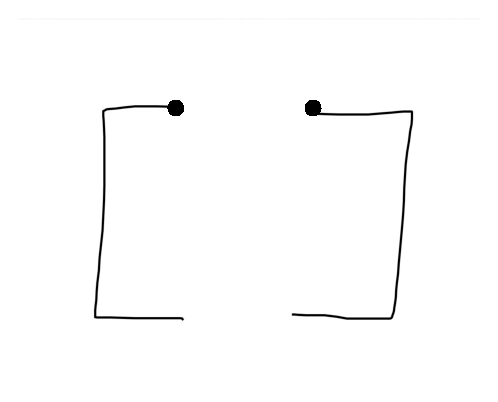
\includegraphics [width=0.5\hsize ]{img/different_direction.eps}
	\end{center}
	\caption{形状が同じであるが書き順の異なる手書きジェスチャの例}
	\label{fig:different_direction}
\end{figure}


\section{スマートフォン以外の端末への応用}
\$Vは,スマートフォンへの手書きジェスチャの入力を想定した,手書きジェスチャ認識アルゴリズムである.
そのため,スマートフォン以外の端末,例えばスマートウォッチやテーブルトップ端末などへの手書きジェスチャの認識アルゴリズムとしても応用できる.
しかしながら,\$1とは違い,大きさ,向き,位置に関して識別可能であるため,それぞれに対する重みを定義する必要がある.
例えば,スマートウォッチはスマートフォンと比べ入力領域が小さいため,大きさや位置の違いを利用しづらく,大きさや位置への重みが小さくなる可能性が高い,反対に,テーブルトップ端末はスマートフォンと比べ入力領域が大きいため,大きさや位置の違いを利用しやすく,大きさや位置への重みが大きくなる可能性が高い.

このように,入力領域を変数として重みを定義することによって,スマートフォン以外の端末への大きさ,向き,位置の違いを利用した手書きジェスチャを認識することが可能になる.

\section{空中手書きジェスチャへの応用}
\$Vは,スマートフォンのような端末への入力を想定しており,認識できる手書きジェスチャは2次元のストロークからなる手書きジェスチャである.これを3次元に応用することによって,Kinectなどの深度センサを用いた~\cite{Tian_kinwrite:handwriting-based}あるいは,端末の加速度を用いた~\cite{Ruiz:2011:UMG:1978942.1978971}ユーザ定義の空中手書きジェスチャを認識することが可能になる.\$3~\cite{Kratz:2010:RSG:1719970.1720051}は\$1を3次元に応用し,空中手書きジェスチャを認識可能にした.このアルゴリズムを活用することによって実現することができる.




%結論
\chapter{結論}
本研究にて,ユーザ定義手書きジェスチャを認識するアルゴリズムである\$Vを開発した.
本論文にてまず,ユーザ調査を行い,アプリケーションユーザは,手書きジェスチャの形状や書き順が同じでも,大きさ,向き,位置の違いを利用したジェスチャを入力したいという要望があることがわかった.これらユーザが定義する手書きジェスチャを認識するためのアルゴリズムを開発した.
\$Vは\$1を拡張し,\$1のように,アルゴリズムが簡潔である,少ない学習データにおいて高い認識率を示す,認識速度が速い,ロバスト性が高いと行った特徴を持ちながら,\$1とは違い,大きさ,向き,位置に関して識別可能にした.
その際,大きさ,向き,位置に関して不変な\$1と比べて,認識速度及び認識率の低下を抑えるために,ジェスチャグループを作成し,類似度計算するジェスチャの数を減らす,かつ保管されている学習データの類似度をもとに,識別するために必要な特徴量を選定するという手法を用いた.
また,識別するために必要な特徴量を選定する上で,それらの特徴量が識別するためにどれくらい必要であるかを重みによって表現することによって,より尤度の高い認識を可能にした.
%アプリケーション開発者は,本論文にて示した.学習データ間の類似度と最適な重みの関係式を用いることによって,そのような認識アルゴリズムを容易に実装できる.

評価実験においては,93\%の認識率を示し,N-best Listの1番目と2番目のスコアの差は0.24であり,高い認識率,識別性能を示した.また,認識速度は\$1と有意差がなく高速であることを示した.また,大きさ,向き,位置が識別可能な既存アルゴリズムと比較し,認識率及び認識速度において高いパフォーマンスを示した.
\$Vは\$1に簡単な数式からなるアルゴリズムを追加するだけであるため,ジェスチャ認識アルゴリズムのライブラリが提供されていない開発環境においても実装可能であるだけでなく,特に手書きジェスチャ認識への深い知識を持たないアプリケーション開発初学者にも,自身のシステムに容易に組み込むことが可能である.
また,\$Vの手書きジェスチャ認識としての改善点及び応用可能性を示した.



\chapter*{謝辞}
\addcontentsline{toc}{chapter}{\numberline{}謝辞}

\newpage

\addcontentsline{toc}{chapter}{\numberline{}参考文献}
\renewcommand{\bibname}{参考文献}

%% 参考文献に jbibtex を使う場合
\bibliographystyle{jalpha}
\bibliography{master_thesis}
%% [compile] jbibtex sample; platex sample; platex sample;

\appendix{}

%\newcommand{\vars}{\texttt}
\let\oldReturn\Return
\renewcommand{\Return}{\State\oldReturn}
\algblockdefx[Foreach]{Foreach}{EndForeach}[1]{\textbf{foreach} #1 \textbf{do}}{\textbf{end foreach}}

\chapter{\$Vアルゴリズムの擬似コード}
\$Vアルゴリズムにおいて,学習データを追加する際のアルゴリズムと,入力データを認識する際のアルゴリズムの擬似コード示す.
本擬似コードにおいて,template\textbf{s}は同じ名前の学習データの集まり,groupは1つのジェスチャグループ,group\textbf{s}は複数のジェスチャグループ~(すなわち全学習データ)を示している.

\begin{algorithm}
  \caption*{\$V-ADD-TEMPLATE(template)}
  \begin{algorithmic}[1]
\State $n\gets 64$
\State $template_\textit{newPoints} \gets REAMPLE(template_\textit{points}, n)$ \Comment{Refer to \$1}
\State $tempate_\textit{size}\gets SIZE(template_\textit{newPoints})$
\State $tempate_\textit{orientation}\gets ORIENTATION(template_\textit{newPoints})$
\State $tempate_\textit{position}\gets POSITION(template_\textit{newPoints})$
\State $<templates, group>\gets SEARCH\mathchar`-SAME\mathchar`-NAME\mathchar`-TEMPLATE(template)$
\If{$templates$}
	\State $templates.push(template)$
	\State $SET\mathchar`-TEMPLATE\mathchar`-FEATURE(templates)$
	\State $SET\mathchar`-GESTURE\mathchar`-GROUP\mathchar`-SIMILARITY(templates, group)$
	\State $SET\mathchar`-GESTURE\mathchar`-GROUP\mathchar`-WEIGHT(group)$
\ElsIf
	\State $<group, score>\gets \$1\mathchar`-RECOGNIZER(template, groups)$
	\If{$score\ge 0.8$}
		\State $templates\gets MAKE\mathchar`-TEMPLATES(template)$
		\State $group.push(templates)$
		\State $SET\mathchar`-GESTURE\mathchar`-GROUP\mathchar`-SIMILARITY(templates, group)$
		\State $SET\mathchar`-GESTURE\mathchar`-GROUP\mathchar`-WEIGHT(group)$
	\ElsIf
		\State $templates\gets MAKE\mathchar`-TEMPLATES(template)$
		\State $group\gets MAKE\mathchar`-GESTURE\mathchar`-GROUP(templates)$
		\State $groups.push(group)$
	\EndIf
\EndIf
\end{algorithmic}
\end{algorithm}

\begin{algorithm}
  \caption*{\$V-RECOGNIZER(gesture, groups)}
  \begin{algorithmic}[1]
  \State $n\gets 64$
  \State $gesture_\textit{newPoints} \gets REAMPLE(template_\textit{points}, n)$ \Comment{Refer to \$1}
  \State $gesture_\textit{size}\gets SIZE(template_\textit{newPoints})$
  \State $gesture_\textit{orientation}\gets ORIENTATION(template_\textit{newPoints})$
  \State $gesutre_\textit{position}\gets POSITION(template_\textit{newPoints})$
  \State $<group, score>\gets \$1\mathchar`-RECOGNIZER(template, groups)$
  \State $bestScore\gets 0$
    \For{$i\gets 1, group_\textit{length}$}
    	\State $templates\gets group_\textit{i}$
	\State $sizeSimilarity\gets SIZE\mathchar`-SIMILARITY(templates_\textit{size}, gesture_\textit{size})$
	\State $\theta 1\gets templates_\textit{orientation}$
	\State $\theta 2\gets gesture_\textit{orientation}$
	\State $orientationSimilarity\gets ORIENTATION\mathchar`-SIMILARITY(\theta 1, \theta 2)$
	\State $x\gets templates_\textit{positionx}$
	\State $x'\gets gesture_\textit{positionx}$
	\State $y\gets templates_\textit{positiony}$
	\State $y'\gets gesture_\textit{positiony}$
	\State $positionSimilarity\gets POSITION\mathchar`-SIMILARITY(x, x', y, y')$
	\State $score\gets sizeSimilarity\times group_\textit{sizeWeight} + orientationSimilarity\times group_\textit{orientationWeight} + positionSimilarity\times group_\textit{positionWeight}$
	\If{$score > bestScore$}
		\State $bestScore\gets score$
		\State $T\gets templates$
	\EndIf
  \EndFor
  \Return <T, score>
\end{algorithmic}
\end{algorithm}


\begin{algorithm}
  \caption*{SET-TEMPLATE-FEATURE(templates)}
  \begin{algorithmic}[1]
  \For{$i\gets 1, templates_\textit{length}$}
  \State $templates_\textit{size}\gets templates_\textit{size} + templates_\textit{isize}$
  \State $templates_\textit{orientation}\gets templates_\textit{orientation} + templates_\textit{iorientation}$
  \State $templates_\textit{positionx}\gets templates_\textit{positionx} + templates_\textit{ipositionx}$
  \State $templates_\textit{positiony}\gets templates_\textit{positiony} + templates_\textit{ipositiony}$
  \EndFor
  \State $templates_\textit{size}\gets templates_\textit{size} / templates_\textit{length}$
  \State $templates_\textit{orientation}\gets templates_\textit{orientation} / templates_\textit{length}$
  \State $templates_\textit{positionx}\gets templates_\textit{positionx} / templates_\textit{length}$
  \State $templates_\textit{positiony}\gets templates_\textit{positiony} / templates_\textit{length}$
\end{algorithmic}
\end{algorithm}

\begin{algorithm}
  \caption*{SET-GESTURE-GROUP-SIMILARITY(templates, group)}
  \begin{algorithmic}[1]
  \State $minSizeSimilarity\gets 1$
   \State $minOrientationSimilarity\gets 1$
    \State $minPositionSimilarity\gets 1$
  \For{$i\gets 1, group_\textit{length}$}
	\State $sizeSimilarity\gets SIZE\mathchar`-SIMILARITY(templates_\textit{size}, group_\textit{isize})$
	\State $minSizeSimilarity\gets MIN(minSizeSimilarity, sizeSimilarity)$
	
	\State $\theta 1\gets templates_\textit{orientation}$
	\State $\theta 2\gets group_\textit{iorientation}$
	\State $orientationSimilarity\gets ORIENTATION\mathchar`-SIMILARITY(\theta 1, \theta 2)$
	%\State $orientationSimilarity\gets ORIENTATION\mathchar`-SIMILARITY(templates_\textit{orientation}, group_\textit{iorientation})$
	\State $minOrientationSimilarity\gets MIN(minOrientationSimilarity, orientationSimilarity)$
	
	\State $x\gets templates_\textit{positionx}$
	\State $x'\gets group_\textit{ipositionx}$
	\State $y\gets templates_\textit{positiony}$
	\State $y'\gets group_\textit{ipositiony}$
	\State $positionSimilarity\gets POSITION\mathchar`-SIMILARITY(x, x', y, y')$
	\State $minPositionSimilarity\gets MIN(minPositionSimilarity, positionSimilarity)$
  \EndFor
  \State $group_\textit{sizeSimilarity}\gets minSizeSimilarity$
  \State $group_\textit{orientationSimilarity}\gets minOrientationSimilarity$
  \State $group_\textit{positionSimilarity}\gets minPostionSimilarity$
\end{algorithmic}
\end{algorithm}

\begin{algorithm}
  \caption*{SIZE-SIMILARITY(size1, size2)}
  \begin{algorithmic}[1]
  \If{$size1\geq size2$}
 		 \State $sizeSimilarity\gets size2 / size1$
	\ElsIf
		\State $sizeSimilarity\gets size1 / size2$
	\EndIf
   \Return sizeSimilarity
\end{algorithmic}
\end{algorithm}

\begin{algorithm}
  \caption*{ORIENTATION-SIMILARITY(orientation1, orientation2)}
  \begin{algorithmic}[1]
  \State $orientationSimilarity\gets ABS(templates_\textit{orientation} - group_\textit{iorientation})$
	\If{$orientationSimilarity > \pi$}
		\State $orientationSimilarity\gets 2\pi - orientationSimilarity$
	\EndIf
	\State $orientationSimilarity\gets 1 - orientationSimilarity / PI$
    \Return orientationSimilarity
\end{algorithmic}
\end{algorithm}

\begin{algorithm}
  \caption*{POSITION-SIMILARITY(x, x', y, y')}
  \begin{algorithmic}[1]
      \State$width\gets inputScreenWidth$
    \State$height\gets inputScreenHeight$
  \State $positionSimilariy\gets 1 - (\sqrt{(x - x')^2 + (y - y')^2} / \sqrt{width^2 + height^2})$
   \Return positionSimilarity
\end{algorithmic}
\end{algorithm}

\begin{algorithm}
  \caption*{SET-GESTURE-GROUP-WEIGHT(group)}
  \begin{algorithmic}[1]
  \State $Ss\gets group_\textit{sizeSimilarity}$
   \State $So\gets group_\textit{orientationSimilarity}$
    \State $Sp\gets group_\textit{positionSimilarity}$
  \State $group_\textit{sizeWeight}\gets (5.5 + 3.5\times (So + Sp) / Ss) / 90$
  \State $group_\textit{orientationWeight}\gets (5.0 + 3.0\times (Ss + Sp) / Sp) / 30$
  \State $group_\textit{positionWeight}\gets (3.0 + 2.0\times (Ss + So) / Sp) / 30$
  \State $sumWeight\gets group_\textit{sizeWeight} + group_\textit{orientationWeight} + group_\textit{positionWeight}$
  \State $group_\textit{sizeWeight}\gets group_\textit{sizeWeight} / sumWeight$
  \State $group_\textit{orientationWeight}\gets group_\textit{orientationWeight} / sumWeight$
  \State $group_\textit{positionWeight}\gets group_\textit{positionWeight} / sumWeight$
\end{algorithmic}
\end{algorithm}

\begin{algorithm}
  \caption*{MAKE-TEMPLATES(template)}
  \begin{algorithmic}[1]
  \State $templates\gets \textbf{new}\: \textbf{TEMPLATES}$
  \State $templates.push(template)$
  \State $templates_\textit{size}\gets - templates_\textit{size}$
  \State $templates_\textit{orienation}\gets - templates_\textit{orientation}$
  \State $templates_\textit{position}\gets - templates_\textit{position}$
  \Return $templates$
\end{algorithmic}
\end{algorithm}

\begin{algorithm}
  \caption*{MAKE-GESTURE-GROUP(templates)}
  \begin{algorithmic}[1]
  %\State $group\gets \textbf{new}\: \textbf{GROUP}$
   \State $group\gets \textbf{new}\: \textbf{GROUP}$
  \State $group.push(templates)$
  \State $group_\textit{sizeSimilarity}\gets -1$
  \State $group_\textit{orientationSimilarity}\gets -1$
  \State $group_\textit{positionSimilarity}\gets -1$
  \State $group_\textit{sizeWeight}\gets 0$
  \State $group_\textit{orientationWeight}\gets 0$
  \State $group_\textit{positionWeight}\gets 0$
  \Return $group$
\end{algorithmic}
\end{algorithm}

\begin{algorithm}
  \caption*{SIZE(points)}
  \begin{algorithmic}[1]
  \State $B\gets BOUNDING\mathchar`-BOX(points)$
  \Return $B_\textit{width} \times B_\textit{height}$
\end{algorithmic}
\end{algorithm}

\begin{algorithm}
  \caption*{ORIENTATION(points)}
  \begin{algorithmic}[1]
  \State $c\gets CENTROID(points)$
  \Return $ATAN(c_\textit{y} - points_\textit{0y}, c_\textit{x} - points_\textit{0x})$
\end{algorithmic}
\end{algorithm}

\begin{algorithm}
  \caption*{POSITION(points)}
  \begin{algorithmic}[1]
  \Return $CENTROID(points)$
\end{algorithmic}
\end{algorithm}

\begin{algorithm}
  \caption*{\$1-RECOGNIZER(gesture, groups)}
  \begin{algorithmic}[1]
  \State $b\gets 0$
  \State $size\gets 250$
  \State $NORMALIZE(gesture)$
  \For{$i\gets 1, groups_\textit{length}$}
  	\State $group\gets groups_\textit{i}$
  	\For{$j\gets 1, group_\textit{length}$}
		\State $templates\gets group_\textit{j}$
		\For{$k\gets 1, templates_\textit{length}$}
			\State $NORMALIZE(templates_\textit{k})$
			\State $d\gets DISTNCE\mathchar`-AT\mathchar`-BEST\mathchar`-ANGLE(gesture, templates_\textit{k})$ \Comment{Refer to \$1}
			\If{d < b}
				\State $b\gets d$
				\State $bestGroup\gets group$
			\EndIf
		\EndFor
	\EndFor
  \EndFor
  \State $score\gets 1 - b / 0.5\sqrt{size^2 + size^2}$
  \Return $<bestGroup, score>$
\end{algorithmic}
\end{algorithm}

\begin{algorithm}
  \caption*{NORMALIZE(template)}
  \begin{algorithmic}[1]
  \State $ROTATE\mathchar`-TO\mathchar`-ZERO(template_\textit{points})$ \Comment{Refer to \$1}
  \State $SCALE\mathchar`-TO\mathchar`-SQUARE(template_\textit{points})$ \Comment{Refer to \$1}
  \State $TRANSLATE\mathchar`-TO\mathchar`-ORIGIN(template_\textit{points})$ \Comment{Refer to \$1}
\end{algorithmic}
\end{algorithm}


%\begin{algorithm}
%  \caption*{RESAMPLE(Points, n)}
%  \begin{algorithmic}[1]
%  \State $I \gets PATH\mathchar`-LENGTH(points) / (n - 1)$
%  \State $D \gets 0$
%  \State $newPoints \gets points_\textit{0}$
%  \For{$i\gets 1, points_\textit{length}$}
%  \If{$(D + d)\ge I$}
%  \State $d \gets DISTANCE(p_\textit{i-1}, p_\textit{i})$
%    \State $q_\textit{x} \gets p_\textit{i-1x} + ((I - D) / d) \times (p_\textit{ix} - p_\textit{i-1x})$
%    \State $q_\textit{y} \gets p_\textit{i-1y} + ((I - D) / d) \times (p_\textit{iy} - p_\textit{i-1y})$
%    \State $APPEND(newPoints, i, q)$ 
%    \State $Insert(points, i, q)$\Comment{q will be the next $p_\textit{i}$}
%    \State $D \gets 0$
%    \Else
%    \State $D \gets D + d$
%    \EndIf
%    \EndFor
%    \Return $newPoints$
%\end{algorithmic}
%\end{algorithm}


%\begin{algorithm}
%  \caption*{PATH-LENGTH(points)}
%  \begin{algorithmic}[1]
%\State $d \gets 0$
%\For{$i\gets 1, points_\textit{length}$}
%\State $d\gets d + DISTANCE(points_\textit{i-1}, points_\textit{i})$
%\EndFor
%\Return d
%\end{algorithmic}
%\end{algorithm}





\end{document}
